%%%%%%%%%%%%%%%%%%%%%%%%%%%%%%%%%%%%
% Slide options
%%%%%%%%%%%%%%%%%%%%%%%%%%%%%%%%%%%%

% Option 1: Slides with solutions

\documentclass[slidestop,compress,mathserif]{beamer}
\newcommand{\soln}[1]{\textit{#1}}
\newcommand{\solnGr}[1]{#1}
\usepackage[T1]{fontenc}
% Option 2: Handouts without solutions

%\documentclass[11pt,containsverbatim,handout]{beamer}
%\usepackage{pgfpages}
%\pgfpagesuselayout{4 on 1}[letterpaper,landscape,border shrink=5mm]
%\newcommand{\soln}[1]{ }
%\newcommand{\solnGr}{ }


%%%%%%%%%%%%%%%%%%%%%%%%%%%%%%%%%%%%
% Style
%%%%%%%%%%%%%%%%%%%%%%%%%%%%%%%%%%%%

\usetheme{metropolis}

%%%%%%%%%%%%%%%%
% Packages
%%%%
%%%%%% pacotes para acentos
%\usepackage[english]{babel}
%\usepackage[latin1]{inputenc}
\usepackage[utf8]{inputenc} 
\usepackage[brazil]{babel}
\usepackage[T1]{fontenc}

\usepackage{geometry}
\usepackage{graphicx}
\usepackage{amssymb}
%\usepackage{cancel}
\usepackage{epstopdf}
\usepackage{amsmath}  	% this permits text in eqnarray among other benefits
\usepackage{url}		% produces hyperlinks
\usepackage{hyperref}	% allows for color usage in tables

\usepackage{colortbl}	% allows for color usage in tables
\usepackage{multirow}	% allows for rows that span multiple rows in tables
\usepackage{color}		% this package has a variety of color options
\usepackage{pgf}
\usepackage{calc}
\usepackage{ulem}
\usepackage{multicol}
\usepackage{textcomp}
\usepackage{txfonts}
\usepackage{listings}
\usepackage{tikz}
\usepackage{array}
\usepackage{wasysym}
\usepackage{fancyvrb}
\usepackage{ragged2e} % justifica o texto
\usepackage{scalefnt} %redimensiona o tamanho da tabela comando = \scalefont{0.5}

%%%%%%%%%%%%%%%%
% Remove navigation symbols
%%%%%%%%%%%%%%%%

\setbeamertemplate{navigation symbols}{}

%%%%%%%%%%%%%%%%
% User defined colors
%%%%%%%%%%%%%%%%

\xdefinecolor{oiB}{rgb}{0.22,0.52,0.72}
\definecolor{oiG}{rgb}{.298,.447,.114}
\xdefinecolor{hlblue}{rgb}{0.051,0.65,1}
\xdefinecolor{gray}{rgb}{0.5, 0.5, 0.5}
\xdefinecolor{darkGray}{rgb}{0.3, 0.3, 0.3}
\xdefinecolor{darkerGray}{rgb}{0.2, 0.2, 0.2}
\xdefinecolor{rubineRed}{rgb}{0.89,0,0.30}
\xdefinecolor{irishGreen}{rgb}{0,0.60,0}	
\definecolor{lightGreen}{rgb}{0.387,0.581,0.148} 

%%%%%%%%%%%%%%%%
% Template colors
%%%%%%%%%%%%%%%%

%\setbeamercolor*{palette primary}{fg=white,bg= oiB!80!black!90}
%\setbeamercolor*{palette secondary}{fg=black,bg= oiB!80!black}
%\setbeamercolor*{palette tertiary}{fg=white,bg= oiB!80!black!80}
%\setbeamercolor*{palette quaternary}{fg=white,bg= oiB}
%\setbeamercolor{structure}{fg= oiB}
%\setbeamercolor{frametitle}{bg= oiB!90}
%\setbeamertemplate{blocks}[shadow=false]
%\setbeamersize{text margin left=2em,text margin right=2em}

%\setbeamercolor{code body}{bg=gray!20!white!80,fg=black}


%%%%%%%%%%%%%%%%
% Get rid of fancy enumerated list bullets
%%%%%%%%%%%%%%%%

%\setbeamertemplate{enumerate items}[default]

%%%%%%%%%%%%%%%%
% Custom commands
%%%%%%%%%%%%%%%%

% degree
\newcommand{\degree}{\ensuremath{^\circ}}

% cite
\newcommand{\ct}[1]{
\vfill
{\tiny #1}}

% Note
\newcommand{\Note}[1]{
\rule{2.5cm}{0.25pt} \\ \textit{\footnotesize{\textcolor{rubineRed}{Note:} \textcolor{darkerGray}{#1}}}}

% Remember
\newcommand{\Remember}[1]{\textit{\scriptsize{\textcolor{orange}{Remember:} #1}}}

% expected counts
\newcommand{\ex}[1]{\textit{\textcolor{blue}{#1}}}

% red
\newcommand{\red}[1]{\textit{\textcolor{rubineRed}{#1}}}

% pink
\newcommand{\pink}[1]{\textit{\textcolor{rubineRed!90!white!50}{#1}}}

% green
\newcommand{\green}[1]{\textit{\textcolor{irishGreen}{#1}}}

% orange
\newcommand{\orange}[1]{\textit{\textcolor{orange}{#1}}}

% links: webURL, webLin, appLink
\newcommand{\webURL}[1]{\urlstyle{same}{ \textit{\textcolor{darkGray}{\url{#1}}}}}
\newcommand{\webLink}[2]{\href{#1}{\textcolor{darkGray}{{#2}}}}
\newcommand{\appLink}[2]{\href{#1}{\textcolor{white}{{#2}}}}

% mail
\newcommand{\mail}[1]{\href{mailto:#1}{\textit{\textcolor{darkGray}{#1}}}}

% highlighting: hl, hlGr, mathhl
\newcommand{\hl}[1]{\textit{\textcolor{hlblue}{#1}}}
\newcommand{\hlGr}[1]{\textit{\textcolor{lightGreen}{#1}}}
\newcommand{\mathhl}[1]{\textcolor{hlblue}{\ensuremath{#1}}}

% two col: two columns
\newenvironment{twocol}[4]{
\begin{columns}[c]
\column{#1\textwidth}
#3
\column{#2\textwidth}
#4
\end{columns}
}

% slot (for probability calculations)
\newenvironment{slot}[2]{
\begin{array}{c} 
\underline{#1} \\ 
#2
\end{array}
}

% pr: left and right parentheses
\newcommand{\pr}[1]{
\left( #1 \right)
}

% solnMult: solutions for practice questions

\newcommand{\solnMult}[1]{
\item[] \vspace{-0.59cm}
\only<1>{\item #1}
\soln{\only<2->{\item \orange{#1}}}
}

% cancel
\newcommand{\cancel}[1]{%
    \tikz[baseline=(tocancel.base)]{
        \node[inner sep=0pt,outer sep=0pt] (tocancel) {#1};
        \draw[red, line width=0.5mm] (tocancel.south west) -- (tocancel.north east);
    }%
}

% removepagenumbers
\newcommand{\removepagenumbers}{% 
  \setbeamertemplate{footline}{}
}

%%%%%%%%%%%%%%%%
% Custom boxes
%%%%%%%%%%%%%%%%

% app: application exercise

\setbeamercolor{app body}{fg=oiG}

\newcommand{\app}[1]{
\begin{beamerboxesrounded}[shadow = false, lower = app body]{}
#1
\end{beamerboxesrounded}
}

% dq: discussion question

\setbeamercolor{disc ques body}{fg=oiB}

\newcommand{\dq}[1]{
\begin{beamerboxesrounded}[shadow = false, lower = disc ques body]{}
#1
\end{beamerboxesrounded}
}

% pq: practice question

\setbeamercolor{prac ques body}{fg=oiB}

\newcommand{\pq}[1]{
\begin{beamerboxesrounded}[shadow = false, lower = prac ques body]{}
#1
\end{beamerboxesrounded}
}

% formula

\setbeamercolor{formula body}{fg=oiB!55!black!95}

\newcommand{\formula}[1]{
\begin{beamerboxesrounded}[shadow = false, lower = formula body]{}
#1
\end{beamerboxesrounded}
}


%%%%%%%%%%%%%%%%
% Change margin
%%%%%%%%%%%%%%%%

\newenvironment{changemargin}[2]{%
\begin{list}{}{%
\setlength{\topsep}{0pt}%
\setlength{\leftmargin}{#1}%
\setlength{\rightmargin}{#2}%
\setlength{\listparindent}{\parindent}%
\setlength{\itemindent}{\parindent}%
\setlength{\parsep}{\parskip}%
}%
\item}{\end{list}}

%%%%%%%%%%%%%%%%
% Footnote
%%%%%%%%%%%%%%%%

\long\def\symbolfootnote[#1]#2{\begingroup%
\def\thefootnote{\fnsymbol{footnote}}\footnote[#1]{#2}\endgroup}

%%%%%%%%%%%%%%%%
% Commands from the book
%%%%%%%%%%%%%%%%

\newenvironment{data}[1]{\texttt{#1}}{}
\newenvironment{var}[1]{\texttt{#1}}{}
\newenvironment{resp}[1]{\texttt{#1}}{}

%%%%%%%%%%%%%%%%
% Graphics
%%%%%%%%%%%%%%%%

\DeclareGraphicsRule{.tif}{png}{.png}{`convert #1 `dirname #1`/`basename #1 .tif`.png}


%%%%%%%%%%%%%%%%%%%%%%%%%%%%%%%%%%%%
% Preamble
%%%%%%%%%%%%%%%%%%%%%%%%%%%%%%%%%%%%

\title[Chp 3: Distributions of RVs]{Capítulo 3: Distribuições de Variáveis Aleatórias}
\institute{$\:$ \\ {\footnotesize Slides desenvolvidos por Mine \c{C}etinkaya-Rundel of OpenIntro. \\
Os slides podem ser copiados, editados e / ou compartilhados via \webLink{http://creativecommons.org/licenses/by-sa/3.0/us/}{CC BY-SA license.} \\
Algumas imagens podem ser incluídas em diretrizes de uso justo (propósitos educacionais).}}
\date{}

%%%%%%%%%%%%%%%%%%%%%%%%%%%%%%%%%%%%
% Begin document
%%%%%%%%%%%%%%%%%%%%%%%%%%%%%%%%%%%%

\begin{document}


%%%%%%%%%%%%%%%%%%%%%%%%%%%%%%%%%%%%
% Title page
%%%%%%%%%%%%%%%%%%%%%%%%%%%%%%%%%%%%

{
\addtocounter{framenumber}{-1} 
{\removepagenumbers 
\usebackgroundtemplate{
\includegraphics[width=\paperwidth]{../OpenIntro_Grid_4_3-01.jpg}}

\begin{frame}


\includegraphics[width=10cm]{../logo_ead.png}

\small	{\textit{Tradução e adaptação: }\\
Priscilla Gnewuch, Márcia Helena Barbian e Maitê Mückler}

\footnotesize{Slides baseados no material desenvolvido por Mine \c{C}etinkaya-Rundel of OpenIntro. }

\footnotesize{Tanto este material  \href{https://github.com/Probabilidade-e-Estatistica-EAD/slides_openintro}{adaptado}, quanto o \href{https://github.com/OpenIntroStat/openintro-statistics-slides}{original}, podem ser copiados, editados e/ou compartilhados. O material adaptado está licenciado sob a Licença Creative Commons Atribuição  4.0 Internacional. Para ver uma cópia desta licença, visite \href{http://creativecommons.org/licenses/by/4.0/} {http://creativecommons.org/licenses/by/4.0/}}


\hfill 
\includegraphics[width=15mm]{../ufrgs-logo}
\includegraphics[width=20mm]{../logoime}
\includegraphics[width=20mm]{../sead-logo}


\end{frame}


\begin{frame}

\titlepage

\end{frame}
}
}


%%%%%%%%%%%%%%%%%%%%%%%%%%%%%%%%%%%%
% Sections
%%%%%%%%%%%%%%%%%%%%%%%%%%%%%%%%%%%%


%%%%%%%%%%%%%%%%%%%%%%%%%%%%%%%%%%%%

\section{3.1. Distribuição normal}

%%%%%%%%%%%%%%%%%%%%%%%%%%%%%%%%%%%%

\begin{frame}
\frametitle{Distribuição normal}

\begin{itemize}
\justifying
\item Curva unimodal e simétrica em forma de sino
\justifying
\item Muitas variáveis são quase normais, mas nenhuma é exatamente normal
\justifying
\item Denotado como \mathhl{N(\mu,\sigma)} $\rightarrow$ Normal com média $\mu$ e desvio padrão $\sigma$

\end{itemize}

\begin{center}
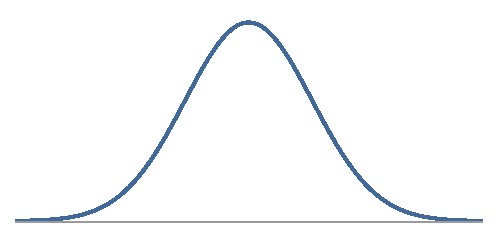
\includegraphics[width=0.7\textwidth]{3-1_normal_distribution/simpleNormal.pdf}
\end{center}

\end{frame}

%%%%%%%%%%%%%%%%%%%%%%%%%%%%%%%%%%%%

\begin{frame}
\frametitle{Alturas dos homens}

\twocol{0.5}{0.5}{
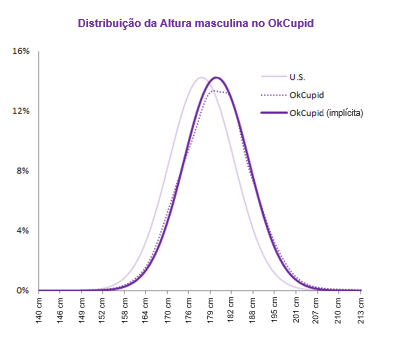
\includegraphics[width=\textwidth]{3-1_normal_distribution/ok_cupid_men.png} \\
}
{
\pause
\justifying
{\footnotesize \\ "As alturas dos homens no OkCupid quase seguem a distribuição normal esperada - exceto pelo fato de que o gráfico é mais deslocado para a direita do que na população geral de homens. Frequentemente os homens gostam de adicionar alguns centímetros à sua altura verdadeira." \\
\justifying
"Uma vaidade discreta pode ser observada: a parte superior da curva pontilhada, que começa em cerca de 176 cm, inclina-se ainda mais para a direita. Isso significa que eles chegam mais perto de um 1 metro e 80 cm, ou seja, aumentando ainda mais o valor de referência da altura desejada pelos homens."
}
}

\ct{\webURL{http://blog.okcupid.com/index.php/the-biggest-lies-in-online-dating/}}

\end{frame}

%%%%%%%%%%%%%%%%%%%%%%%%%%%%%%%%%%%%

\begin{frame}
\frametitle{Alturas das mulheres}

\twocol{0.5}{0.5}{
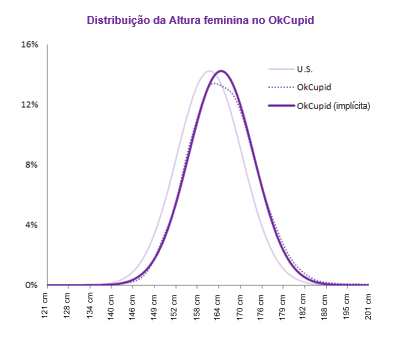
\includegraphics[width=\textwidth]{3-1_normal_distribution/ok_cupid_women.png} \\
}
{
\pause
\justifying
{\footnotesize \\" Já quando analisamos os dados das mulheres, ficamos surpresos ao ver que o exagero da altura uma característica tão propagada, embora, no caso das mulheres, sem necessariamente uma altura de referência desejada."
}
}

\vfill
\justifying
\ct{\webURL{http://blog.okcupid.com/index.php/the-biggest-lies-in-online-dating/}}

\end{frame}

%%%%%%%%%%%%%%%%%%%%%%%%%%%%%%%%%%%%

\subsection{Modelo de distribuição normal}

%%%%%%%%%%%%%%%%%%%%%%%%%%%%%%%%%%%%

\begin{frame}
\frametitle{Distribuições normais com diferentes parâmetros}

\vspace{-0.5cm}
\begin{center}
$\mu$: média, $\sigma$: desvio padrão
\[N(\mu = 0, \sigma = 1) \hspace{1.4cm} N(\mu = 19, \sigma = 4) \]
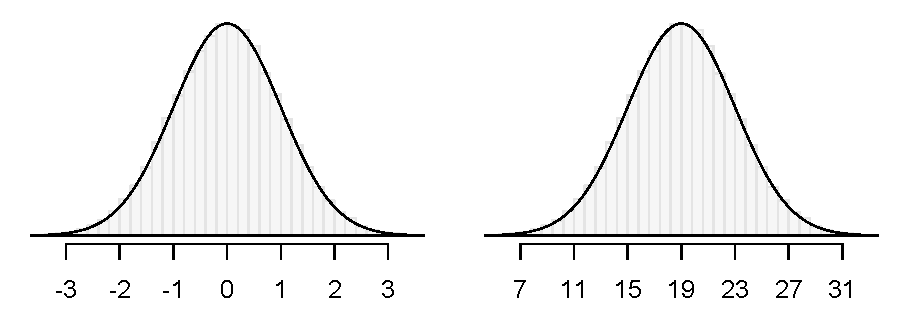
\includegraphics[width=0.6\textwidth]{3-1_normal_distribution/twoSampleNormals.pdf} \\
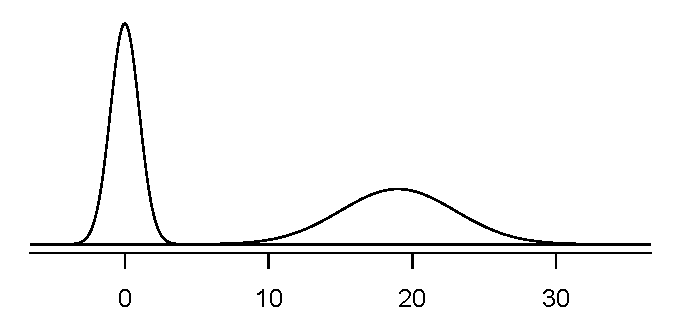
\includegraphics[width=0.6\textwidth]{3-1_normal_distribution/twoSampleNormalsStacked.pdf}
\end{center}

\end{frame}

%%%%%%%%%%%%%%%%%%%%%%%%%%%%%%%%%%%%

\subsection{Padronizando com escores Z}

%%%%%%%%%%%%%%%%%%%%%%%%%%%%%%%%%%%%

\begin{frame}
\frametitle{Distribuições normais com diferentes parâmetros}
\justifying
\dq{\footnotesize Os escores do SAT (\textit{Scholastic Aptitude Test} - um tipo de vestibular americano) possuem distribuição quase normal, com média 1.500 e desvio padrão 300. Os escores do ACT (\textit{American College Testing} - outro vestibular americano) também são distribuídos quase que normalmente, com média 21 e desvio padrão 5. 

\\ Um funcionário responsável pela aprovação dos candidatos em uma Universidade gostaria de determinar qual, de dois candidatos, obteve uma pontuação melhor em seu vestibular em relação aos outros vestibulandos: Pam, que obteve 1800 em seu SAT, ou Jim, que marcou 24 em seu ACT?}

\begin{center}
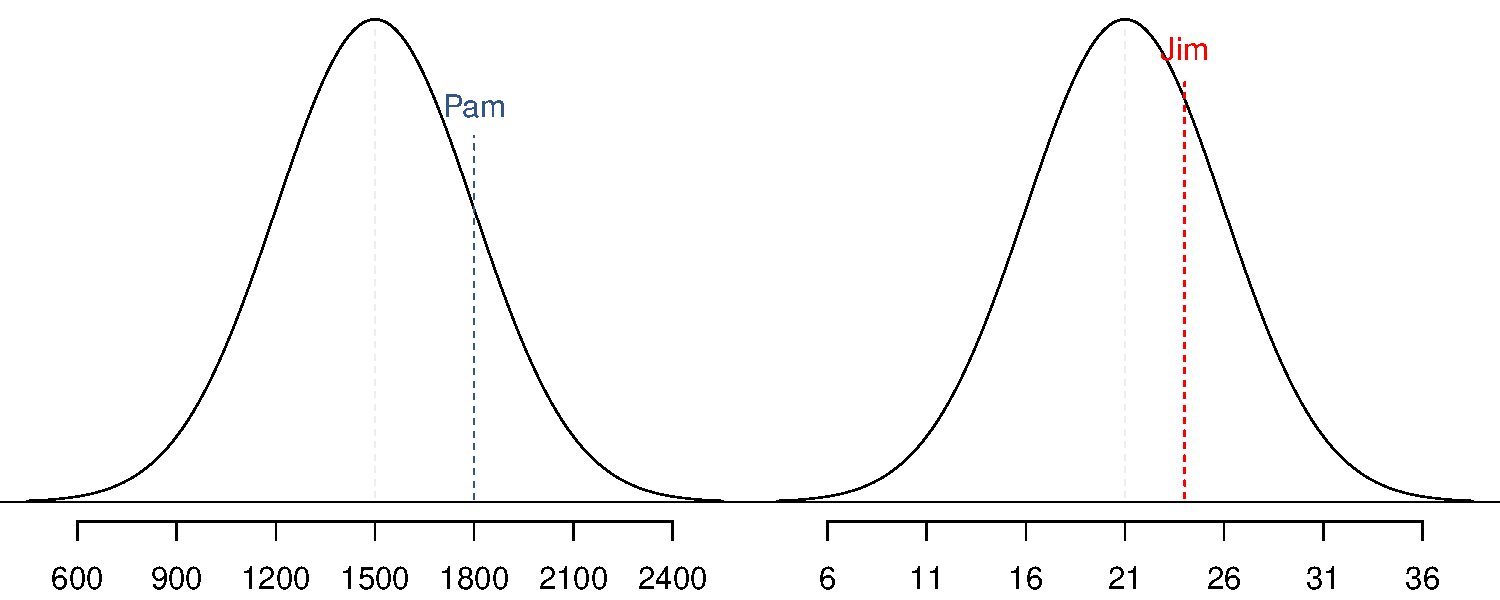
\includegraphics[width=0.8\textwidth]{3-1_normal_distribution/satActNormals.pdf}
\end{center}

\end{frame}

%%%%%%%%%%%%%%%%%%%%%%%%%%%%%%%%%%%%

\begin{frame}
\frametitle{Padronizando com escores Z}
\justifying
Como não podemos simplesmente comparar esses dois escores brutos, vamos verificar a quantos desvios-padrão além da média cada escore está.

\begin{itemize}
\justifying
\item A pontuação de Pam é $\frac{1800 - 1500}{300} = 1$ desvio padrão acima da média.
\justifying
\item A pontuação de Jim é $\frac{24 - 21}{5} = 0.6$ desvios-padrão acima da média.

\end{itemize}

\begin{center}
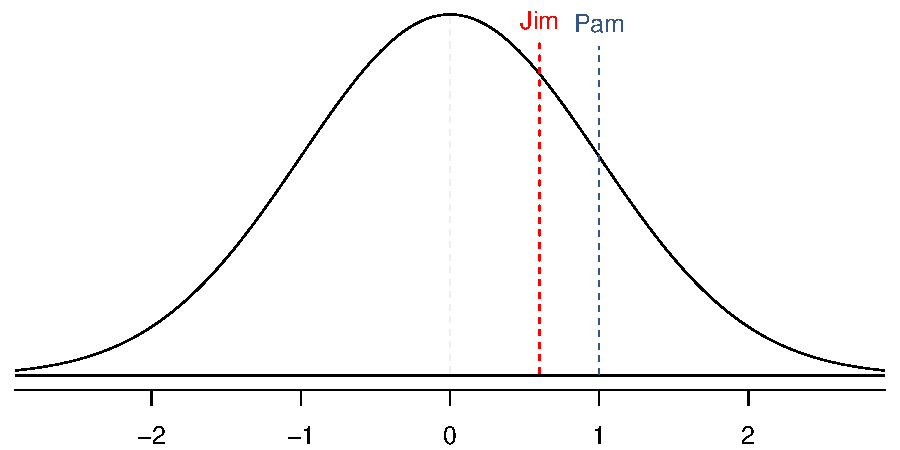
\includegraphics[width=0.6\textwidth]{3-1_normal_distribution/satActNormalsStandardized.pdf}
\end{center}

\end{frame}

%%%%%%%%%%%%%%%%%%%%%%%%%%%%%%%%%%%%

\begin{frame}
\frametitle{Padronizando com escores Z (cont.)}

\begin{itemize}
\justifying
\item Estes são chamados de \hl{escores padronizado}, ou \hl{escores Z}.
\justifying
\item O escore Z de uma observação é o número de desvios-padrão que esta observação está acima ou abaixo da média.\\
\formula{\[Z = \frac{observacao - media}{SD}\]}
\justifying
\item Os escores Z são definidos para distribuições de qualquer formato, porém somente quando a distribuição é normal podemos usar escores Z para calcular \hl{percentis}.
\justifying
\item Observações que estão a mais de 2 desvios-padrão da média ($ | Z |> 2 $) são geralmente consideradas incomuns.

\end{itemize}

\end{frame}

%%%%%%%%%%%%%%%%%%%%%%%%%%%%%%%%%%%%

\begin{frame}
\frametitle{Percentis}

\begin{itemize}
\justifying
\item \hl{Percentil} é a porcentagem de observações que caem abaixo de um determinado valor da distribuição de dados.
\justifying
\item Graficamente, o percentil é a área abaixo da curva de distribuição de probabilidade à esquerda dessa observação.

\end{itemize}

\begin{center}
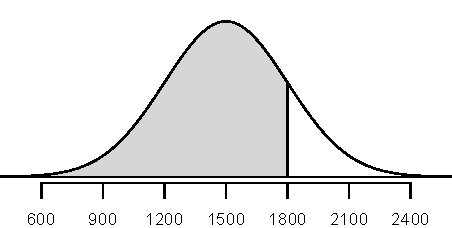
\includegraphics[width=0.7\textwidth]{3-1_normal_distribution/satBelow1800.pdf}
\end{center}

\end{frame}

%%%%%%%%%%%%%%%%%%%%%%%%%%%%%%%%%%%%

\begin{frame}
\frametitle{Percentis}
\justifying
\dq{Aproximadamente, qual porcentagem de alunos tem pontuação abaixo de 1800 no SAT? (Dica: use a regra 68-95-99.7\%.)}

\only<1>{
\begin{center}
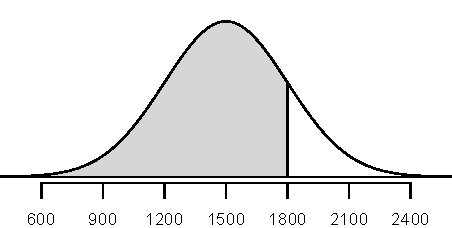
\includegraphics[width=0.7\textwidth]{3-1_normal_distribution/satBelow1800.pdf}
\end{center}
}

\only<2 | handout:0>{
\begin{center}
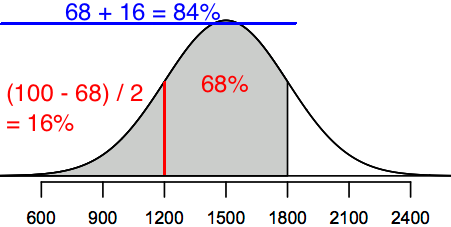
\includegraphics[width=0.7\textwidth]{3-1_normal_distribution/satBelow1800_soln.png}
\end{center}
}
\vspace{-0.5cm}
\soln{\only<2>{
\begin{align*}
100 - 68 &= 32\% \\
32 / 2 &= 16\% \\
68 + 16 &= 84\%
\end{align*}}}

\end{frame}
%
%%%%%%%%%%%%%%%%%%%%%%%%%%%%%%%%%%%%%

\subsection{Tabela de probabilidade normal}

%%%%%%%%%%%%%%%%%%%%%%%%%%%%%%%%%%%%

\begin{frame}[fragile]
\frametitle{Calculando percentis - usando computação}
\justifying
Existem muitas maneiras de calcular os percentis/áreas sob a curva:

\begin{itemize}
\item R:
\end{itemize}
\begin{beamerboxesrounded}[shadow = false, lower = code body]{}
{\small \begin{verbatim}
> pnorm(1800, mean = 1500, sd = 300)
[1] 0.8413447
\end{verbatim}
}
\end{beamerboxesrounded}
\begin{itemize}
\item Applet: {\small \webURL{https://gallery.shinyapps.io/dist_calc/}}
\begin{center}
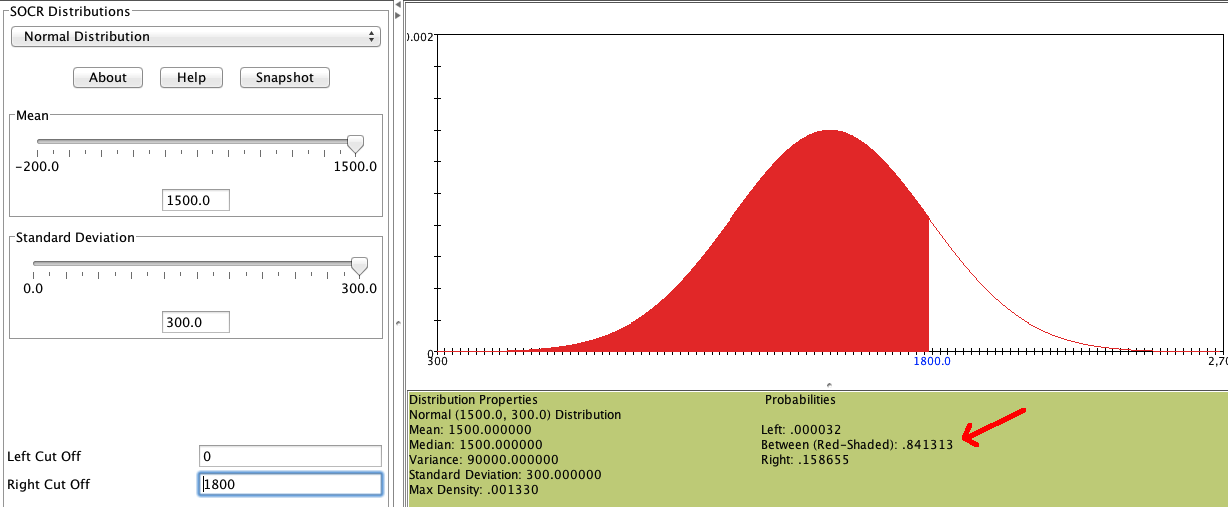
\includegraphics[width=0.8\textwidth]{3-1_normal_distribution/applet.png}
\end{center}

\end{itemize}


\end{frame}

%%%%%%%%%%%%%%%%%%%%%%%%%%%%%%%%%%%%

\begin{frame}[fragile]
\frametitle{Calculando percentis - usando tabelas}

{\footnotesize
\begin{tabular}{c | >{\columncolor[gray]{0.6}[0pt]}rrrrr | rrrrr |}
  \cline{2-11}
&&&& \multicolumn{4}{c}{Second decimal place of $Z$} &&& \\
  \cline{2-11}
$Z$ & 0.00 & 0.01 & 0.02 & 0.03 & 0.04 & 0.05 & 0.06 & 0.07 & 0.08 & 0.09 \\
  \hline
  \hline
0.0 & \tiny{0.5000} & \tiny{0.5040} & \tiny{0.5080} & \tiny{0.5120} & \tiny{0.5160} & \tiny{0.5199} & \tiny{0.5239} & \tiny{0.5279} & \tiny{0.5319} & \tiny{0.5359} \\
  0.1 & \tiny{0.5398} & \tiny{0.5438} & \tiny{0.5478} & \tiny{0.5517} & \tiny{0.5557} & \tiny{0.5596} & \tiny{0.5636} & \tiny{0.5675} & \tiny{0.5714} & \tiny{0.5753} \\
  0.2 & \tiny{0.5793} & \tiny{0.5832} & \tiny{0.5871} & \tiny{0.5910} & \tiny{0.5948} & \tiny{0.5987} & \tiny{0.6026} & \tiny{0.6064} & \tiny{0.6103} & \tiny{0.6141} \\
  0.3 & \tiny{0.6179} & \tiny{0.6217} & \tiny{0.6255} & \tiny{0.6293} & \tiny{0.6331} & \tiny{0.6368} & \tiny{0.6406} & \tiny{0.6443} & \tiny{0.6480} & \tiny{0.6517} \\
  0.4 & \tiny{0.6554} & \tiny{0.6591} & \tiny{0.6628} & \tiny{0.6664} & \tiny{0.6700} & \tiny{0.6736} & \tiny{0.6772} & \tiny{0.6808} & \tiny{0.6844} & \tiny{0.6879} \\
  \hline
  0.5 & \tiny{0.6915} & \tiny{0.6950} & \tiny{0.6985} & \tiny{0.7019} & \tiny{0.7054} & \tiny{0.7088} & \tiny{0.7123} & \tiny{0.7157} & \tiny{0.7190} & \tiny{0.7224} \\
  0.6 & \tiny{0.7257} & \tiny{0.7291} & \tiny{0.7324} & \tiny{0.7357} & \tiny{0.7389} & \tiny{0.7422} & \tiny{0.7454} & \tiny{0.7486} & \tiny{0.7517} & \tiny{0.7549} \\
  0.7 & \tiny{0.7580} & \tiny{0.7611} & \tiny{0.7642} & \tiny{0.7673} & \tiny{0.7704} & \tiny{0.7734} & \tiny{0.7764} & \tiny{0.7794} & \tiny{0.7823} & \tiny{0.7852} \\
  0.8 & \tiny{0.7881} & \tiny{0.7910} & \tiny{0.7939} & \tiny{0.7967} & \tiny{0.7995} & \tiny{0.8023} & \tiny{0.8051} & \tiny{0.8078} & \tiny{0.8106} & \tiny{0.8133} \\
  0.9 & \tiny{0.8159} & \tiny{0.8186} & \tiny{0.8212} & \tiny{0.8238} & \tiny{0.8264} & \tiny{0.8289} & \tiny{0.8315} & \tiny{0.8340} & \tiny{0.8365} & \tiny{0.8389} \\
  \hline
  \hline
\rowcolor[gray]{.6}
  1.0 & \orange{\tiny{0.8413}} & \tiny{0.8438} & \tiny{0.8461} & \tiny{0.8485} & \tiny{0.8508} & \tiny{0.8531} & \tiny{0.8554} & \tiny{0.8577} & \tiny{0.8599} & \tiny{0.8621} \\
  1.1 & \tiny{0.8643} & \tiny{0.8665} & \tiny{0.8686} & \tiny{0.8708} & \tiny{0.8729} & \tiny{0.8749} & \tiny{0.8770} & \tiny{0.8790} & \tiny{0.8810} & \tiny{0.8830} \\
  1.2 & \tiny{0.8849} & \tiny{0.8869} & \tiny{0.8888} & \tiny{0.8907} & \tiny{0.8925} & \tiny{0.8944} & \tiny{0.8962} & \tiny{0.8980} & \tiny{0.8997} & \tiny{0.9015} \\
\end{tabular}
}

\end{frame}

%%%%%%%%%%%%%%%%%%%%%%%%%%%%%%%%%%%%

\subsection{Exemplos de probabilidade normal}

%%%%%%%%%%%%%%%%%%%%%%%%%%%%%%%%%%%%

\begin{frame}
\frametitle{6 sigma}
\justifying
``O termo \textit {processo 6 sigma} vem da ideia de que, se houver seis desvios-padrão entre a média do processo e o limite de especificação mais próximo, como mostrado no gráfico, praticamente nenhum item deixará de atender às especificações."

\begin{center}
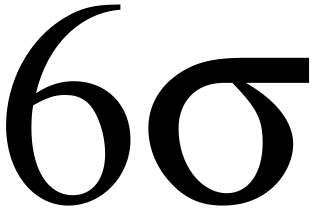
\includegraphics[width=0.35\textwidth]{3-1_normal_distribution/sixsigma.png}
\end{center}

\ct{\webURL{http://en.wikipedia.org/wiki/Six_Sigma}}

\end{frame}

%%%%%%%%%%%%%%%%%%%%%%%%%%%%%%%%%%%%

\begin{frame}
\frametitle{Controle de qualidade}
\justifying
\dq{{\small Na fábrica de ketchup Heinz, as quantidades de ketchup inseridas nas garrafas devem ser normalmente distribuídas com uma média de 36g e desvio-padrão 0,11g. A cada 30 minutos, uma garrafa é selecionada da linha de produção e seu conteúdo é precisamente anotado. Se a quantidade de ketchup na garrafa estiver abaixo de 35,8g ou acima de 36,2g, então o frasco falha na inspeção de controle de qualidade. Qual a porcentagem de garrafas possue menos de 35,8g de ketchup?}}

\soln{\pause
\centering Seja $X$ = quantidade de ketchup em uma garrafa: \\ $X \sim N(\mu = 36, \sigma = 0,11)$ \\
\pause
\twocol{0.4}{0.6}{
\begin{center}
\centering
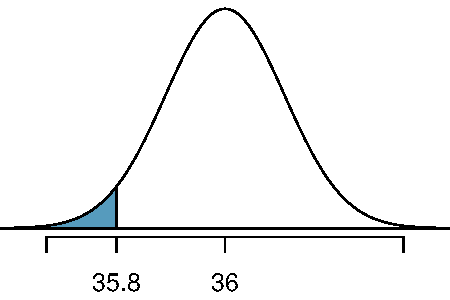
\includegraphics[width=\textwidth]{3-1_normal_distribution/ketchupLT358.pdf}
\end{center}
}
{
\pause
\[ Z = \frac{35.8 - 36}{0.11} = -1.82 \]
}
}

\end{frame}

%%%%%%%%%%%%%%%%%%%%%%%%%%%%%%%%%%%%

\begin{frame}
\frametitle{Encontrar a probabilidade exata - usando a tabela Z}

\only<1>{
{\footnotesize
\begin{tabular}{| rrrrr | rrrrr | c}
  \cline{1-10}
&&& \multicolumn{4}{c}{Segunda casa decimal de $ Z $} &&& \\
  \cline{1-10}
0.09 &  0.08 &  0.07 &  0.06 &  0.05 &  0.04 &  0.03 &  0.02 &  0.01 &  0.00 & $Z$  \\
    \hline
    \hline
  \tiny{0.0014} & \tiny{0.0014} & \tiny{0.0015} & \tiny{0.0015} & \tiny{0.0016} & \tiny{0.0016} & \tiny{0.0017} & \tiny{0.0018} & \tiny{0.0018} & \tiny{0.0019} & $-2.9$ \\
  \tiny{0.0019} & \tiny{0.0020} & \tiny{0.0021} & \tiny{0.0021} & \tiny{0.0022} & \tiny{0.0023} & \tiny{0.0023} & \tiny{0.0024} & \tiny{0.0025} & \tiny{0.0026} & $-2.8$ \\
  \tiny{0.0026} & \tiny{0.0027} & \tiny{0.0028} & \tiny{0.0029} & \tiny{0.0030} & \tiny{0.0031} & \tiny{0.0032} & \tiny{0.0033} & \tiny{0.0034} & \tiny{0.0035} & $-2.7$ \\
  \tiny{0.0036} & \tiny{0.0037} & \tiny{0.0038} & \tiny{0.0039} & \tiny{0.0040} & \tiny{0.0041} & \tiny{0.0043} & \tiny{0.0044} & \tiny{0.0045} & \tiny{0.0047} & $-2.6$ \\
  \tiny{0.0048} & \tiny{0.0049} & \tiny{0.0051} & \tiny{0.0052} & \tiny{0.0054} & \tiny{0.0055} & \tiny{0.0057} & \tiny{0.0059} & \tiny{0.0060} & \tiny{0.0062} & $-2.5$ \\
    \hline
  \tiny{0.0064} & \tiny{0.0066} & \tiny{0.0068} & \tiny{0.0069} & \tiny{0.0071} & \tiny{0.0073} & \tiny{0.0075} & \tiny{0.0078} & \tiny{0.0080} & \tiny{0.0082} & $-2.4$ \\
  \tiny{0.0084} & \tiny{0.0087} & \tiny{0.0089} & \tiny{0.0091} & \tiny{0.0094} & \tiny{0.0096} & \tiny{0.0099} & \tiny{0.0102} & \tiny{0.0104} & \tiny{0.0107} & $-2.3$ \\
  \tiny{0.0110} & \tiny{0.0113} & \tiny{0.0116} & \tiny{0.0119} & \tiny{0.0122} & \tiny{0.0125} & \tiny{0.0129} & \tiny{0.0132} & \tiny{0.0136} & \tiny{0.0139} & $-2.2$ \\
  \tiny{0.0143} & \tiny{0.0146} & \tiny{0.0150} & \tiny{0.0154} & \tiny{0.0158} & \tiny{0.0162} & \tiny{0.0166} & \tiny{0.0170} & \tiny{0.0174} & \tiny{0.0179} & $-2.1$ \\
  \tiny{0.0183} & \tiny{0.0188} & \tiny{0.0192} & \tiny{0.0197} & \tiny{0.0202} & \tiny{0.0207} & \tiny{0.0212} & \tiny{0.0217} & \tiny{0.0222} & \tiny{0.0228} & $-2.0$ \\
    \hline
  \tiny{0.0233} & \tiny{0.0239} & \tiny{0.0244} & \tiny{0.0250} & \tiny{0.0256} & \tiny{0.0262} & \tiny{0.0268} & \tiny{0.0274} & \tiny{0.0281} & \tiny{0.0287} & $-1.9$ \\
  \tiny{0.0294} & \tiny{0.0301} & \tiny{0.0307} & \tiny{0.0314} & \tiny{0.0322} & \tiny{0.0329} & \tiny{0.0336} & \tiny{0.0344} & \tiny{0.0351} & \tiny{0.0359} & $-1.8$ \\
  \tiny{0.0367} & \tiny{0.0375} & \tiny{0.0384} & \tiny{0.0392} & \tiny{0.0401} & \tiny{0.0409} & \tiny{0.0418} & \tiny{0.0427} & \tiny{0.0436} & \tiny{0.0446} & $-1.7$ \\
  \tiny{0.0455} & \tiny{0.0465} & \tiny{0.0475} & \tiny{0.0485} & \tiny{0.0495} & \tiny{0.0505} & \tiny{0.0516} & \tiny{0.0526} & \tiny{0.0537} & \tiny{0.0548} & $-1.6$ \\
  \tiny{0.0559} & \tiny{0.0571} & \tiny{0.0582} & \tiny{0.0594} & \tiny{0.0606} & \tiny{0.0618} & \tiny{0.0630} & \tiny{0.0643} & \tiny{0.0655} & \tiny{0.0668} & $-1.5$ \\
\hline
\end{tabular}
}}

\soln{
\only<2|folheto:0>{
{\scalefont{0.6}
\begin{tabular}{| rrrrr | rr>{\columncolor[gray]{0.6}[0pt]}rrr | c}
  \cline{1-10}
&&& \multicolumn{4}{c}{Segunda casa decimal de $ Z $} &&& \\
  \cline{1-10}
0.09 &  0.08 &  0.07 &  0.06 &  0.05 &  0.04 &  0.03 &  0.02 &  0.01 &  0.00 & $Z$  \\
    \hline
    \hline
  \tiny{0.0014} & \tiny{0.0014} & \tiny{0.0015} & \tiny{0.0015} & \tiny{0.0016} & \tiny{0.0016} & \tiny{0.0017} & \tiny{0.0018} & \tiny{0.0018} & \tiny{0.0019} & $-2.9$ \\
  \tiny{0.0019} & \tiny{0.0020} & \tiny{0.0021} & \tiny{0.0021} & \tiny{0.0022} & \tiny{0.0023} & \tiny{0.0023} & \tiny{0.0024} & \tiny{0.0025} & \tiny{0.0026} & $-2.8$ \\
  \tiny{0.0026} & \tiny{0.0027} & \tiny{0.0028} & \tiny{0.0029} & \tiny{0.0030} & \tiny{0.0031} & \tiny{0.0032} & \tiny{0.0033} & \tiny{0.0034} & \tiny{0.0035} & $-2.7$ \\
  \tiny{0.0036} & \tiny{0.0037} & \tiny{0.0038} & \tiny{0.0039} & \tiny{0.0040} & \tiny{0.0041} & \tiny{0.0043} & \tiny{0.0044} & \tiny{0.0045} & \tiny{0.0047} & $-2.6$ \\
  \tiny{0.0048} & \tiny{0.0049} & \tiny{0.0051} & \tiny{0.0052} & \tiny{0.0054} & \tiny{0.0055} & \tiny{0.0057} & \tiny{0.0059} & \tiny{0.0060} & \tiny{0.0062} & $-2.5$ \\
    \hline
  \tiny{0.0064} & \tiny{0.0066} & \tiny{0.0068} & \tiny{0.0069} & \tiny{0.0071} & \tiny{0.0073} & \tiny{0.0075} & \tiny{0.0078} & \tiny{0.0080} & \tiny{0.0082} & $-2.4$ \\
  \tiny{0.0084} & \tiny{0.0087} & \tiny{0.0089} & \tiny{0.0091} & \tiny{0.0094} & \tiny{0.0096} & \tiny{0.0099} & \tiny{0.0102} & \tiny{0.0104} & \tiny{0.0107} & $-2.3$ \\
  \tiny{0.0110} & \tiny{0.0113} & \tiny{0.0116} & \tiny{0.0119} & \tiny{0.0122} & \tiny{0.0125} & \tiny{0.0129} & \tiny{0.0132} & \tiny{0.0136} & \tiny{0.0139} & $-2.2$ \\
  \tiny{0.0143} & \tiny{0.0146} & \tiny{0.0150} & \tiny{0.0154} & \tiny{0.0158} & \tiny{0.0162} & \tiny{0.0166} & \tiny{0.0170} & \tiny{0.0174} & \tiny{0.0179} & $-2.1$ \\
  \tiny{0.0183} & \tiny{0.0188} & \tiny{0.0192} & \tiny{0.0197} & \tiny{0.0202} & \tiny{0.0207} & \tiny{0.0212} & \tiny{0.0217} & \tiny{0.0222} & \tiny{0.0228} & $-2.0$ \\
    \hline
  \tiny{0.0233} & \tiny{0.0239} & \tiny{0.0244} & \tiny{0.0250} & \tiny{0.0256} & \tiny{0.0262} & \tiny{0.0268} & \tiny{0.0274} & \tiny{0.0281} & \tiny{0.0287} & $-1.9$ \\
\rowcolor[gray]{.6}
  \tiny{0.0294} & \tiny{0.0301} & \tiny{0.0307} & \tiny{0.0314} & \tiny{0.0322} & \tiny{0.0329} & \tiny{0.0336} & \orange{\tiny{0.0344}} & \tiny{0.0351} & \tiny{0.0359} & $-1.8$ \\
  \tiny{0.0367} & \tiny{0.0375} & \tiny{0.0384} & \tiny{0.0392} & \tiny{0.0401} & \tiny{0.0409} & \tiny{0.0418} & \tiny{0.0427} & \tiny{0.0436} & \tiny{0.0446} & $-1.7$ \\
  \tiny{0.0455} & \tiny{0.0465} & \tiny{0.0475} & \tiny{0.0485} & \tiny{0.0495} & \tiny{0.0505} & \tiny{0.0516} & \tiny{0.0526} & \tiny{0.0537} & \tiny{0.0548} & $-1.6$ \\
  \tiny{0.0559} & \tiny{0.0571} & \tiny{0.0582} & \tiny{0.0594} & \tiny{0.0606} & \tiny{0.0618} & \tiny{0.0630} & \tiny{0.0643} & \tiny{0.0655} & \tiny{0.0668} & $-1.5$ \\
\hline
\end{tabular}
}}}

\end{frame}

%%%%%%%%%%%%%%%%%%%%%%%%%%%%%%%%%%%%

\begin{frame}[fragile]
\frametitle{Encontrar a probabilidade exata - usando R}

\begin{beamerboxesrounded}[shadow = true, lower = code body]{}
{\small \begin{verbatim}
> pnorm(-1.82, mean = 0, sd = 1)
[1] 0.0344
\end{verbatim}
}
\end{beamerboxesrounded}

$\:$ \\
\pause

ou

$\:$ \\
\pause

\begin{beamerboxesrounded}[shadow = true, lower = code body]{}
{\small \begin{verbatim}
> pnorm(35.8, mean = 36, sd = 0.11)
[1] 0.0345
\end{verbatim}
}
\end{beamerboxesrounded}


\end{frame}
%
%%%%%%%%%%%%%%%%%%%%%%%%%%%%%%%%%%%%%

\begin{frame}
\frametitle{Prática}
\justifying
\pq{Qual o percentual de garrafas que \underline {passa} na inspeção de controle de qualidade?}

\vspace{-0.5cm}
\begin{multicols}{2}
\begin{enumerate}[(a)]
\item 1.82\%
\item 3.44\%
\item 6.88\%
\solnMult{93.12\%}
\item 96.56\%
\item[]
\end{enumerate}
\end{multicols}

\soln{
\vspace{-0.5cm}
\pause
\begin{columns}[c]
\column{0.3\textwidth}
\pause
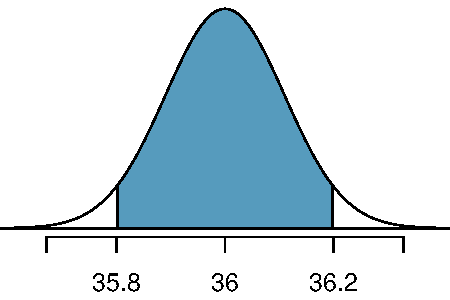
\includegraphics[width=\textwidth]{3-1_normal_distribution/ketchupBET.pdf}
\column{0.05\textwidth}
=
\pause
\column{0.3\textwidth}
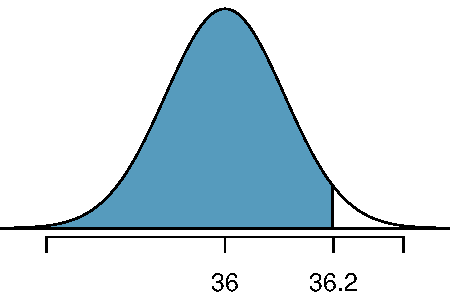
\includegraphics[width=\textwidth]{3-1_normal_distribution/ketchupLT362.pdf}
\column{0.05\textwidth}
-
\pause
\column{0.3\textwidth}
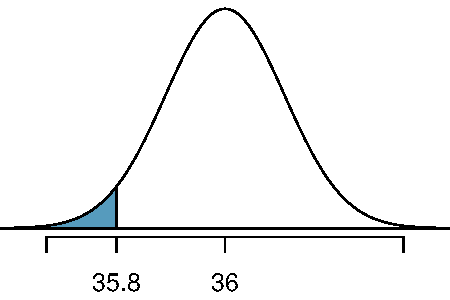
\includegraphics[width=\textwidth]{3-1_normal_distribution/ketchupLT358.pdf}
\end{columns}
\pause
\scalefont{0.8}
\begin{eqnarray*}
Z_{35.8} &=& \frac{35.8 - 36}{0.11} = -1.82 \\ \pause
Z_{36.2} &=& \frac{36.2 - 36}{0.11} = 1.82 \\ \pause
P(35.8 < X < 36.2) &=& P(-1.82 < Z < 1.82) = 0.9656 - 0.0344 = 0.9312
\end{eqnarray*}
}

\end{frame}

%%%%%%%%%%%%%%%%%%%%%%%%%%%%%%%%%%%%

\begin{frame}
\frametitle{Encontrando pontos de corte}
\justifying
\dq{\footnotesize Em seres humanos saudáveis, as temperaturas corporais são distribuídas quase que normalmente com média 98,2$^{\circ}$ F e desvio-padrão de 0,73$^{\circ}$ F. \\ Qual é o ponto de corte dos 3\% que possuem temperaturas corporais mais baixas?}

\pause

\twocol{0.35}{0.65}
{
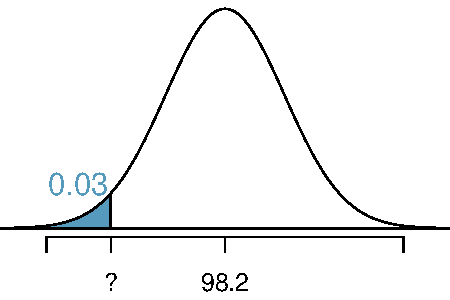
\includegraphics[width=\textwidth]{3-1_normal_distribution/tempLOW3PERC.pdf}
}
{
\pause
{\footnotesize
\begin{tabular}{| r >{\columncolor[gray]{0.9}[0pt]}rrrr | c |}
\hline
0.09 &  0.08 &  0.07 &  0.06 &  0.05 & $Z$  \\
    \hline
    \hline
  \tiny{0.0233} & \tiny{0.0239} & \tiny{0.0244} & \tiny{0.0250} & \tiny{0.0256} & $-1.9$ \\
  \rowcolor[gray]{.9}
  \tiny{0.0294} & \tiny{\orange{0.0301}} & \tiny{0.0307} & \tiny{0.0314} & \tiny{0.0322} &$-1.8$ \\
  \tiny{0.0367} & \tiny{0.0375} & \tiny{0.0384} & \tiny{0.0392} & \tiny{0.0401} &$-1.7$ \\
\hline
\end{tabular}
}
}
\pause
\begin{eqnarray*}
P(X < x) &=& 0.03 \rightarrow P(Z < \orange{-1.88}) = 0.03 \\ \pause
Z &=& \frac{obs~-~media}{SD} \rightarrow \frac{x - 98.2}{0.73} = -1.88 \\ \pause
x &=& (-1.88 \times 0.73) + 98.2 = 96.8\degree F
\end{eqnarray*}

\ct{Mackowiak, Wasserman, and Levine (1992), \textit{Uma avaliação crítica de 98,6 graus F, o limite superior da temperatura corporal normal e outros legados de Carl Reinhold August Wunderlick}.}

\end{frame}

%%%%%%%%%%%%%%%%%%%%%%%%%%%%%%%%%%%%

\begin{frame}
\frametitle{Prática}
\justifying
\pq{\footnotesize Em seres humanos saudáveis, as temperaturas corporais são distribuídas quase que normalmente com média 98,2$^{\circ}$ F e desvio-padrão de 0,73$^{\circ}$ F. \\ Qual é o ponto de corte dos 10\% que possuem temperaturas corporais mais altas?}

\vspace{-0.5cm}
\begin{multicols}{2}
\begin{enumerate}[(a)]
\item 97.3$\degree$F
\solnMult{99.1$\degree$F}
\item 99.4$\degree$F
\item 99.6$\degree$F
\end{enumerate}
\end{multicols}

\soln{
\vspace{-0.5cm}
\pause
\twocol{0.35}{0.65}
{
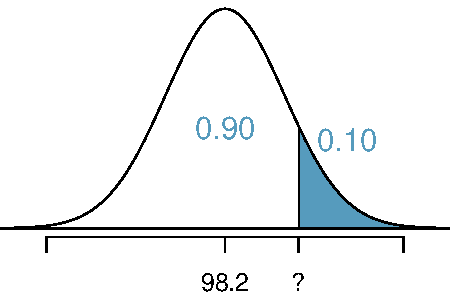
\includegraphics[width=\textwidth]{3-1_normal_distribution/tempHIGH10PERC.pdf}
}
{
\pause
{\footnotesize
\begin{tabular}{|c | rrr >{\columncolor[gray]{0.9}[0pt]}rr |}
\hline
$Z$ & 0.05 & 0.06 & 0.07 & 0.08 & 0.09 \\
  \hline
  \hline
  1.0 & \tiny{0.8531} & \tiny{0.8554} & \tiny{0.8577} & \tiny{0.8599} & \tiny{0.8621} \\
  1.1  & \tiny{0.8749} & \tiny{0.8770} & \tiny{0.8790} & \tiny{0.8810} & \tiny{0.8830} \\
   \rowcolor[gray]{.9}
 1.2 & \tiny{0.8944} & \tiny{0.8962} & \tiny{0.8980} & \tiny{\orange{0.8997}} & \tiny{0.9015} \\
  1.3 & \tiny{0.9115} & \tiny{0.9131} & \tiny{0.9147} & \tiny{0.9162} & \tiny{0.9177} \\
   \hline
\end{tabular}
}
}
}
\pause
\scalefont{0.6}
\begin{eqnarray*}
P(X > x) &=& 0.10 \rightarrow P(Z < \orange{1.28}) = 0.90 \\ \pause
Z &=& \frac{obs~-~media}{SD} \rightarrow \frac{x - 98.2}{0.73} = 1.28 \\ \pause
x &=& (1.28 \times 0.73) + 98.2 = 99.1
\end{eqnarray*}

\end{frame}

%%%%%%%%%%%%%%%%%%%%%%%%%%%%%%%%%%%%

\subsection{Regra 68-95-99.7}

%%%%%%%%%%%%%%%%%%%%%%%%%%%%%%%%%%%%

\begin{frame}
\frametitle{Regra 68-95-99.7}

\begin{itemize}
\justifying
\item Para dados quase normalmente distribuídos, 
\begin{itemize}
\justifying
\item cerca de 68 \% cai dentro de 1 SD da média,
\justifying
\item cerca de 95 \% cai dentro de 2 SD da média,
\justifying
\item cerca de 99,7 \% cai dentro de 3 SD da média.
\end{itemize}
\justifying
\item É possível que as observações caiam 4, 5 ou mais desvios-padrão da média, mas essas ocorrências são muito raras se os dados forem quase normais.

\end{itemize}

\begin{center}
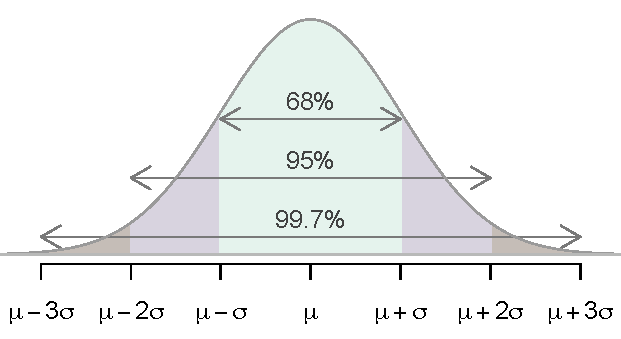
\includegraphics[width=0.7\textwidth]{3-1_normal_distribution/6895997.pdf}
\end{center}

\end{frame}

%%%%%%%%%%%%%%%%%%%%%%%%%%%%%%%%%%%%

\begin{frame}
\frametitle{Descrevendo a variabilidade usando a regra 68-95-99.7}
\justifying
Os escores do SAT são distribuídos quase que normalmente com média 1.500 e desvio padrão 300.

\pause
\begin{itemize}
\justifying
\footnotesize
\item $\sim$68\% dos alunos possuem pontuação entre 1200 e 1800 no SAT.
\justifying
\item $\sim$95\% dos alunos possuem pontuação entre 900 e 2100 no SAT. 
\justifying
\item $\sim$99.7\% dos alunos possuem pontuação entre 600 e 2400 no SAT. 

\end{itemize}

\begin{center}
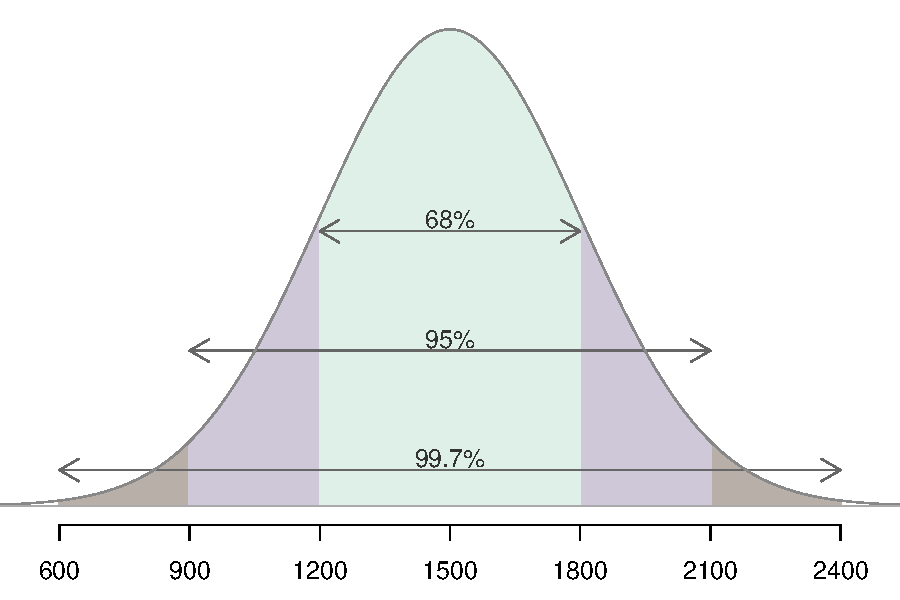
\includegraphics[width=0.65\textwidth]{3-1_normal_distribution/sat_empirical.pdf}
\end{center}

\end{frame}

%%%%%%%%%%%%%%%%%%%%%%%%%%%%%%%%%%%%

\begin{frame}[fragile]
\frametitle{Número de horas de sono de estudantes}

\only<1 | handout:0>{
\begin{center}
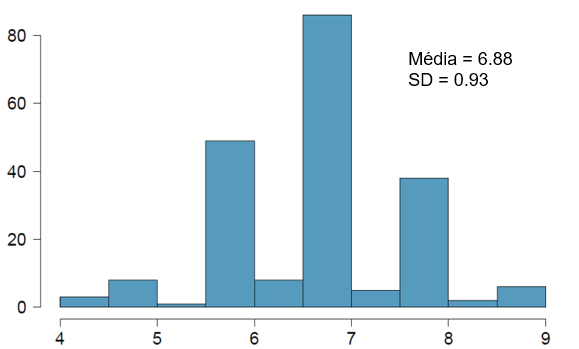
\includegraphics[width=0.75\textwidth]{3-1_normal_distribution/sleep-hist.png} 
\end{center}
\vspace{-0.25cm}
\begin{itemize}
\item Média = 6.88 horas, SD = 0.92 horas
\item[] \textcolor{white}{72\% dos dados estão dentro de 1 SD da média: $6.88 \pm 0.93$}
\item[] \textcolor{white}{92\% dos dados estão dentro de 1 SD da média: $6.88 \pm 2 \times 0.93$}
\item[] \textcolor{white}{99\% dos dados estão dentro de 1 SD da média: $6.88 \pm 3 \times 0.93$}
\end{itemize}
}

\only<2 | handout:0>{
\begin{center}
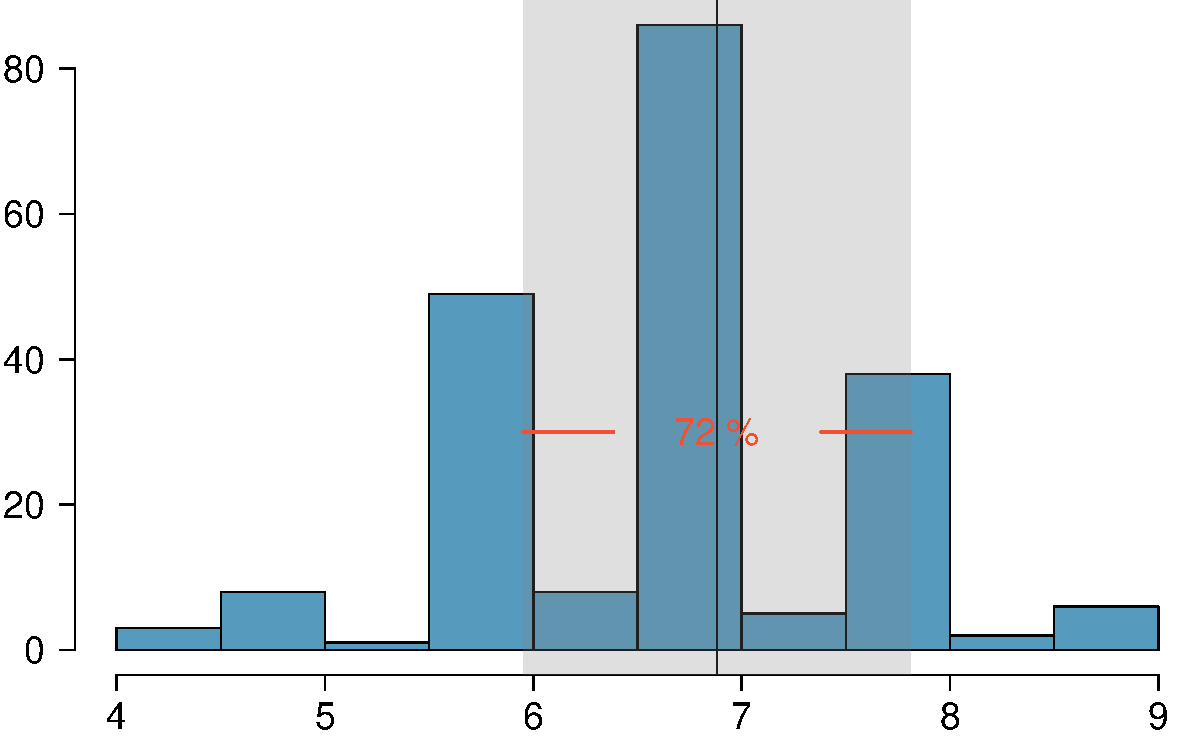
\includegraphics[width=0.75\textwidth]{3-1_normal_distribution/sleep-hist-sd1.pdf} 
\end{center}
\vspace{-0.25cm}
\begin{itemize}
\justifying
\item Média = 6.88 horas, SD = 0.92 horas
\justifying
\item 72\% dos dados estão dentro de 1 SD da média: $6.88 \pm 0.93$
\justifying
\item[] \textcolor{white}{92\% dos dados estão dentro de 1 SD da média: $6.88 \pm 2 \times 0.93$}
\justifying
\item[] \textcolor{white}{99\% dos dados estão dentro de 1 SD da média: $6.88 \pm 3 \times 0.93$}
\end{itemize}
}

\only<3 | handout:0>{
\begin{center}
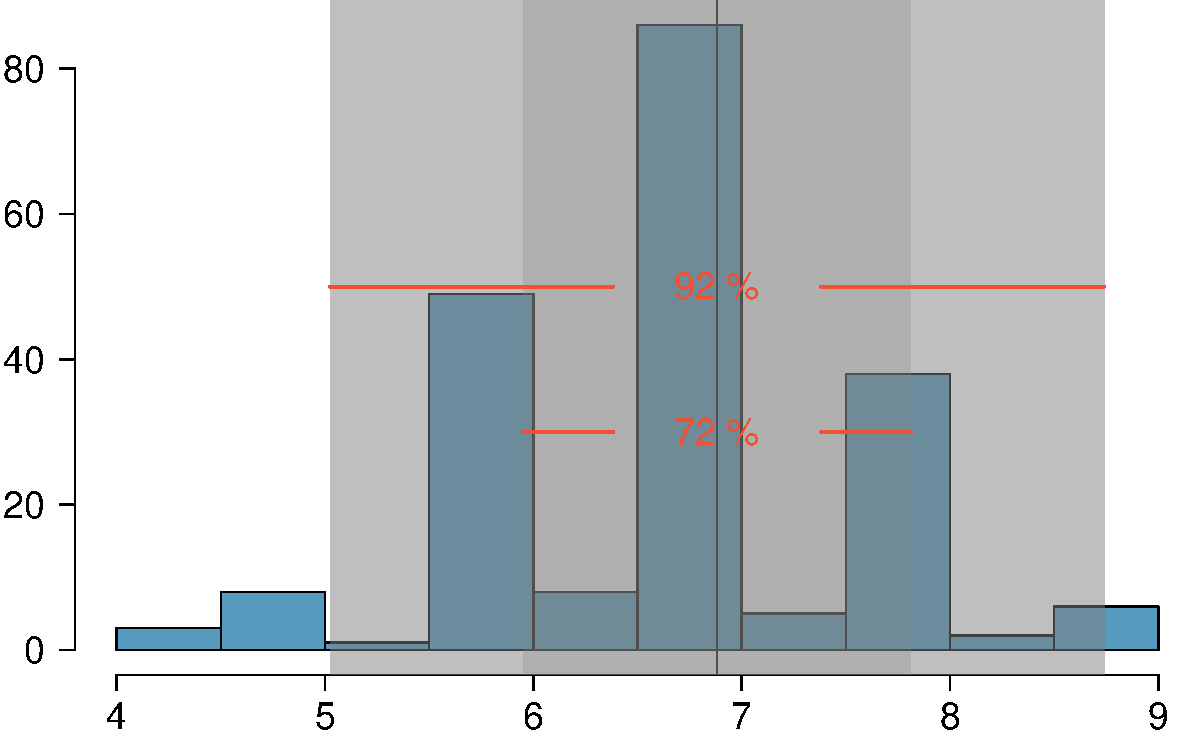
\includegraphics[width=0.75\textwidth]{3-1_normal_distribution/sleep-hist-sd2.pdf} 
\end{center}
\vspace{-0.25cm}
\begin{itemize}
\justifying
\item Média = 6.88 horas, SD = 0.92 horas
\justifying
\item 72\% dos dados estão dentro de 1 SD da média: $6.88 \pm 0.93$
\justifying
\item 92\% dos dados estão dentro de 1 SD da média: $6.88 \pm 2 \times 0.93$
\justifying
\item[] \textcolor{white}{99\% dos dados estão dentro de 1 SD da média: $6.88 \pm 3 \times 0.93$}
\end{itemize}
}

\only<4>{
\begin{center}
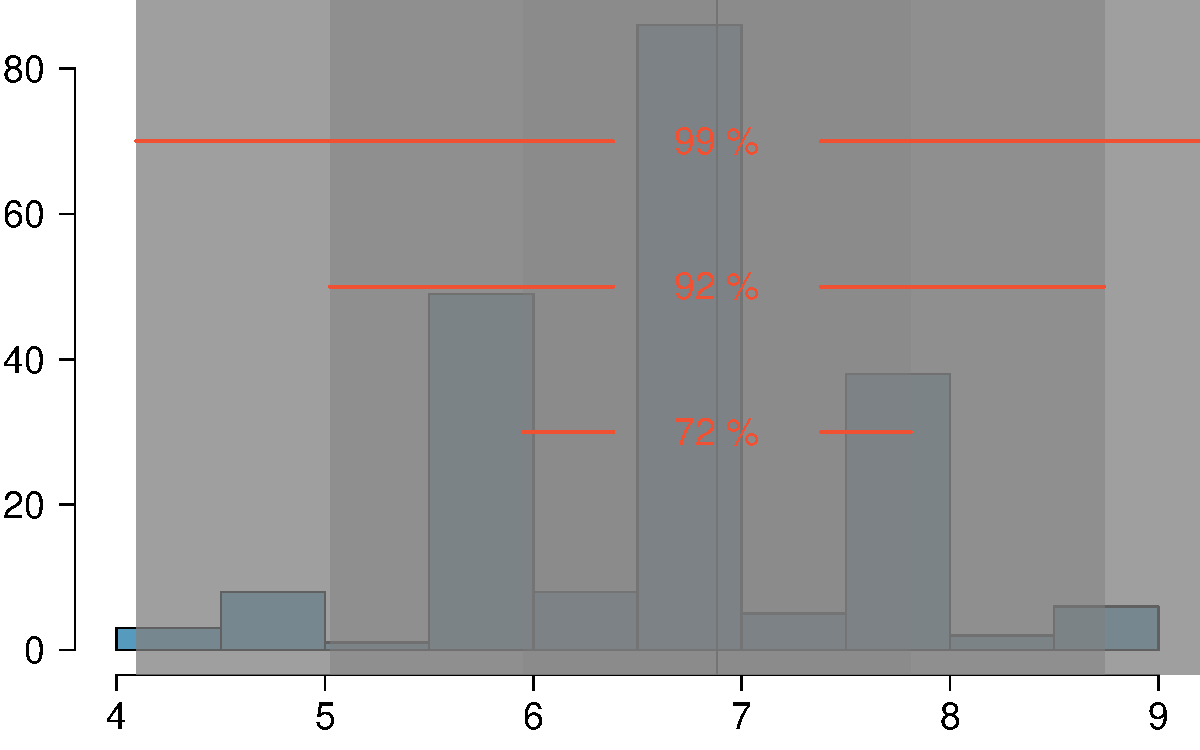
\includegraphics[width=0.75\textwidth]{3-1_normal_distribution/sleep-hist-sd3.pdf} 
\end{center}
\vspace{-0.2cm}
\small{
\begin{itemize}
\justifying
\item Média = 6.88 horas, SD = 0.92 horas
\justifying
\item 72\% dos dados estão dentro de 1 SD da média: $6.88 \pm 0.93$
\justifying
\item 92\% dos dados estão dentro de 1 SD da média: $6.88 \pm 2 \times 0.93$
\justifying
\item 99\% dos dados estão dentro de 1 SD da média: $6.88 \pm 3 \times 0.93$
\end{itemize}
}}

\end{frame}

%%%%%%%%%%%%%%%%%%%%%%%%%%%%%%%%%%%%

\begin{frame}
\frametitle{Prática}
\justifying
\pq{Qual das seguintes opções é \underline{falsa}?}

\begin{enumerate}[(a)]
\justifying
\item A maioria dos escores Z de uma distribuição assimétrica à direita são negativos.
\justifying
\solnMult{Em distribuições assimétricas, o escore Z da média pode ser diferente de 0.}
\justifying
\item Para uma distribuição normal, o IQR é inferior a $2 \times SD$.
\justifying
\item Os escores Z são úteis para determinar o quão incomum é um ponto de dados quando comparado ao restante dos dados da distribuição.
\end{enumerate}

\end{frame}

%%%%%%%%%%%%%%%%%%%%%%%%%%%%%%%%%%%%


%%%%%%%%%%%%%%%%%%%%%%%%%%%%%%%%%%%%

\section{3.2. Avaliando a aproximação normal}

%%%%%%%%%%%%%%%%%%%%%%%%%%%%%%%%%%%%

\subsection{Gráfico de probabilidade normal}

%%%%%%%%%%%%%%%%%%%%%%%%%%%%%%%%%%%%

\begin{frame}
\frametitle{Gráfico de probabilidade normal}
\justifying
Um histograma e um \hl {gráfico de probabilidade normal} de uma amostra de 100 alturas masculinas.

\begin{center}
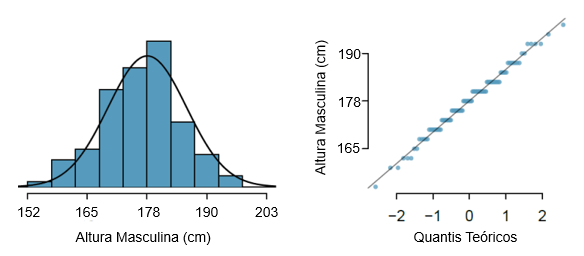
\includegraphics[width=0.9\textwidth]{3-2_evaluating_normal_approx/fcidMHeights.png}
\end{center}

\end{frame}

%%%%%%%%%%%%%%%%%%%%%%%%%%%%%%%%%%%%

\begin{frame}
\frametitle{Anatomia de um gráfico de probabilidade normal}

\begin{itemize}
\justifying
\item Os dados são plotados no eixo y de um gráfico de probabilidade normal e quantis teóricos (seguindo uma distribuição normal) no eixo x.
\justifying
\item Se houver um relacionamento linear no gráfico, os dados seguem uma distribuição quase normal.
\justifying
\item A construção de um gráfico de probabilidade normal requer o cálculo dos percentis e dos escores z correspondentes para cada observação, o que pode ser entediante. Portanto, geralmente dependemos de um software para fazer esses gráficos.

\end{itemize}

\end{frame}

%%%%%%%%%%%%%%%%%%%%%%%%%%%%%%%%%%%%

\begin{frame}
\frametitle{Exemplo}
\justifying
\dq{Abaixo está um histograma e um gráfico de probabilidade normal para as alturas da NBA da temporada 2008-2009. Esses dados parecem seguir uma distribuição normal?}

\begin{center}
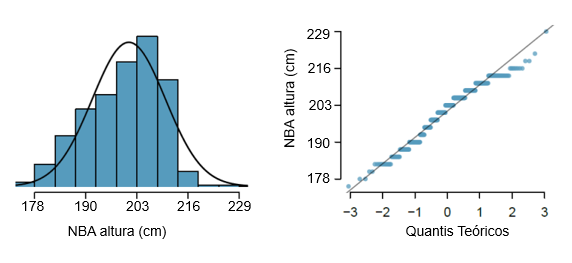
\includegraphics[width=0.8\textwidth]{3-2_evaluating_normal_approx/nbaNormal.png}
\end{center}

\pause
\justifying
\dq{Por que os pontos de probabilidade normal têm saltos?}

\end{frame}

%%%%%%%%%%%%%%%%%%%%%%%%%%%%%%%%%%%%

\begin{frame}
\frametitle{Gráfico de probabilidade normal e assimetria}

\twocol{0.2}{0.8}{
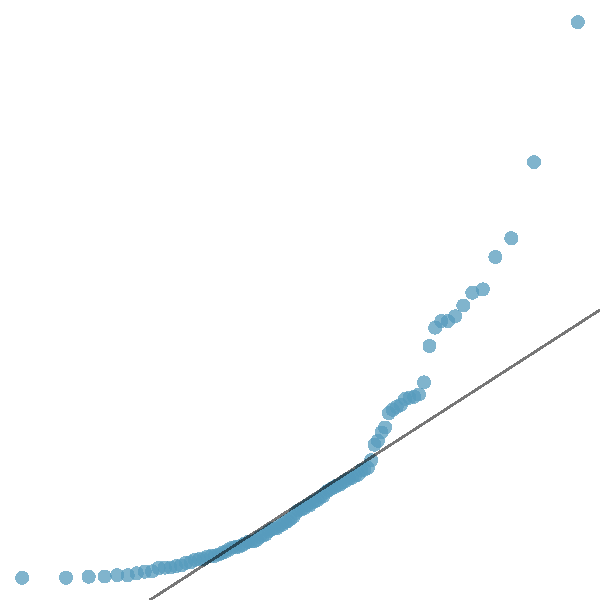
\includegraphics[width=0.8\textwidth]{3-2_evaluating_normal_approx/qq_rs.pdf}
}
{
\justifying
Inclinação à direita - Os pontos são curvados para cima e para a esquerda da linha.
}

\twocol{0.2}{0.8}{
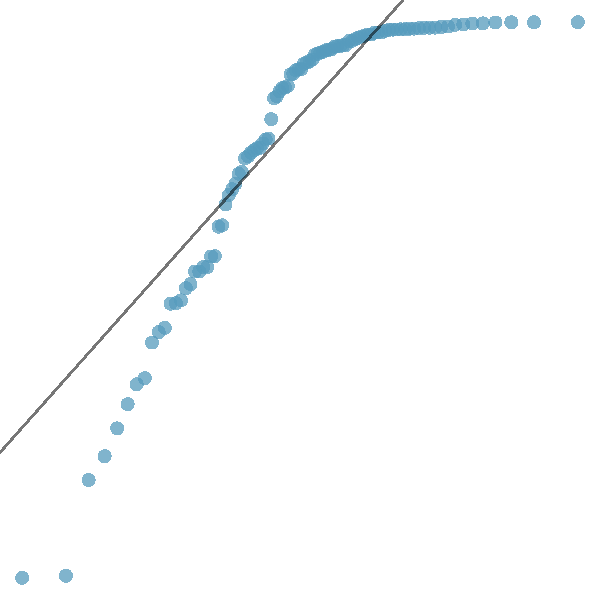
\includegraphics[width=0.8\textwidth]{3-2_evaluating_normal_approx/qq_ls.pdf}
}
{
\justifying
Inclinação da esquerda - Pontos curvados para baixo e para a direita da linha.
}

\twocol{0.2}{0.8}{
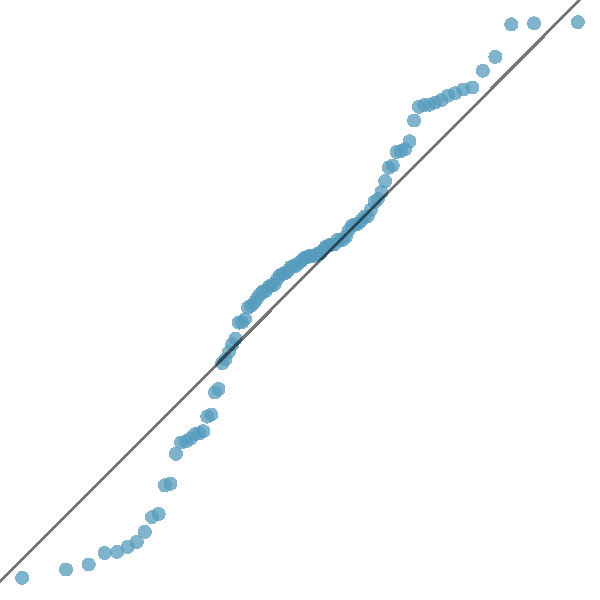
\includegraphics[width=0.8\textwidth]{3-2_evaluating_normal_approx/qq_st.pdf}
}
{
\justifying
Inclinação mais acentuada (mais estreitas que a distribuição normal) - Os pontos seguem uma curva em forma de S.
}

\twocol{0.2}{0.8}{
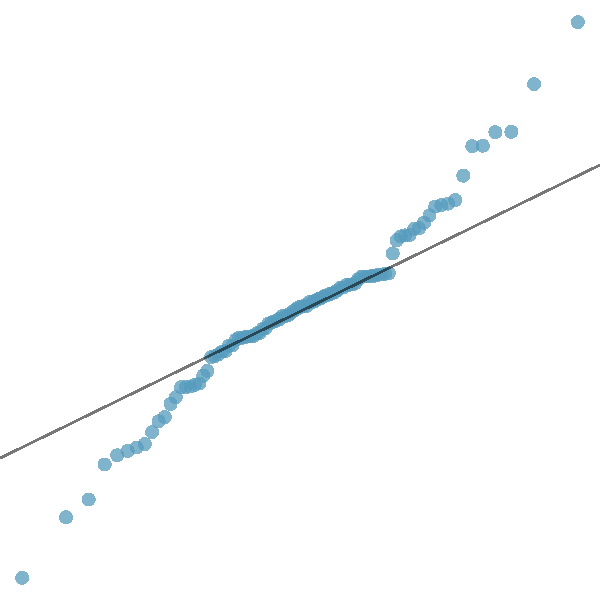
\includegraphics[width=0.8\textwidth]{3-2_evaluating_normal_approx/qq_lt.pdf}
}
{
\justifying
Inclinação menos acentuada (mais largas que a distribuição normal) - Os pontos começam abaixo da linha, passando a seguir a linha e terminam acima dela linha.
}

\end{frame}

%%%%%%%%%%%%%%%%%%%%%%%%%%%%%%%%%%%%


%%%%%%%%%%%%%%%%%%%%%%%%%%%%%%%%%%%%

\section{3.3. Distribuição geométrica}

%%%%%%%%%%%%%%%%%%%%%%%%%%%%%%%%%%%%

\subsection{Distribuição Bernoulli}

\begin{frame}
\frametitle{Experimento de Milgram}

\twocol{0.6}{0.4}{

\begin{itemize}
\justifying
\item Stanley Milgram, psicólogo da Universidade de Yale, conduziu uma série de experimentos sobre obediência à autoridade a partir de 1963.
\justifying
\item O pesquisador (E) ordena que o professor (T), que é o sujeito do experimento, aplique choques elétricos a um aluno (L) toda vez que este responder a uma pergunta incorretamente.

\end{itemize}

}
{
\begin{center}
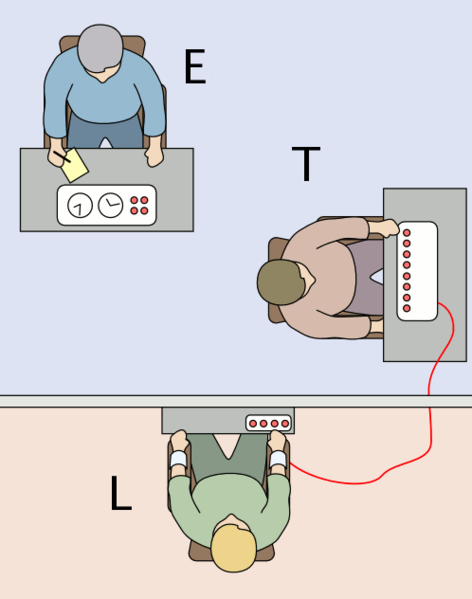
\includegraphics[width=\textwidth]{3-3_geometric_distribution/milgram.png}
\end{center}
\justifying
\ct{\webURL{http://en.wikipedia.org/wiki/File:Milgram_Experiment_v2.png}}
}

\end{frame}


%%%%%%%%%%%%%%%%%%%%%%%%%%%%%%%%%%%%

\begin{frame}
\frametitle{Experimento de Milgram (cont.)}

\begin{itemize}
\justifying
\item O aluno é na verdade um ator, e os choques elétricos não são reais, mas um som pré-gravado é tocado toda vez que o professor administra um choque elétrico.
\justifying
\item Esse experimento mediu a vontade dos participantes do estudo em obedecer a uma figura de autoridade que os instruiu a realizar atos que conflitassem com sua consciência pessoal.
\justifying
\item Milgram descobriu que cerca de 65\% das pessoas obedeceriam à autoridade e dariam tais choques.
\justifying
\item Ao longo dos anos, outras pesquisas sugeriram que esse número é aproximadamente consistente entre as comunidades e o tempo.

\end{itemize}

\end{frame}


%%%%%%%%%%%%%%%%%%%%%%%%%%%%%%%%%%%%

\begin{frame}
\frametitle{Variáveis aleatórias de Bernoulli}

\begin{itemize}
\justifying
\item Na experiência de Milgram cada pessoa pode ser tratada como uma \hl{tentativa}.
\justifying
\item A pessoa é considerada como \hl{sucesso} se ela se recusar a administrar um choque e como \hl{falha} se ela administrar o choque.
\justifying
\item Como apenas 35\% das pessoas se recusaram a administrar o choque, a \hl{probabilidade de sucesso} é \mathhl{p = 0.35}.
\justifying
\item Quando uma particular tentativa tem apenas dois resultados possíveis, ela é chamada de \hl{variável aleatória de Bernoulli}.

\end{itemize}

\end{frame}

%%%%%%%%%%%%%%%%%%%%%%%%%%%%%%%%%%%%

\subsection{Distribuição geométrica}

\begin{frame}
\frametitle{Distribuição geométrica}

{\small
\justifying
\dq{A Dra. Smith quer repetir os experimentos de Milgram, mas ela só quer testar pessoas até encontrar alguém que não esteja disposto a aplicar choques. Qual é a probabilidade de ela parar o experimento depois da primeira pessoa?}

\[ P(1^{0}~pessoa~recusa) = 0.35 \]

\pause
\justifying
\dq{... a terceira pessoa?}
\[ P(1^{0}~e~2^{0}~choque,~3^{0}~recusa) = \slot{S}{0.65} \times \slot{S}{0.65} \times  \slot{R}{0.35} = 0.65^2 \times 0.35 \approx 0.15 \]
}
\pause
\end{frame}

%%%%%%%%%%%%%%%%%%%%%%%%%%%%%%%%%%%%

\begin{frame}
\frametitle{Distribuição geométrica}
{\small
\dq{... a décima pessoa?}
\soln{
\pause
\[ P(9~choque,~10^{0}~recusa) = \underbrace{\slot{S}{0.65} \times \cdots \times \slot{S}{0.65}}_{9~deste} \times  \slot{R}{0.35} = 0.65^9 \times 0.35 \approx 0.0072 \]
}
}

\end{frame}

%%%%%%%%%%%%%%%%%%%%%%%%%%%%%%%%%%%%

\begin{frame}
\frametitle{Distribuição geométrica (cont.)}
\justifying
A \hl{Distribuição geométrica} descreve o tempo de espera até um sucesso para variáveis aleatórias Bernoulli \hl{independentes e identicamente distribuídas (iid)}.
\pause
\begin{itemize}
\justifying
\item independência: os resultados dos ensaios não afetam uns aos outros.
\justifying
\item idêntico: a probabilidade de sucesso é a mesma para cada tentativa.
\end{itemize}
\pause
\formula{Probabilidades geométricas}{Se $ p $ representa a probabilidade de sucesso, então $ (1-p) $ representa a probabilidade de falha e $ n $ representa número de tentativas independentes \[P(sucesso~na~n^{esima}~tentativa) = (1-p)^{n-1} p\]}

\end{frame}
%%%%%%%%%%%%%%%%%%%%%%%%%%%%%%%%%%%%


\begin{frame}
\frametitle{Exemplo}
\justifying
\pq{Podemos calcular a probabilidade de obter um 6 pela primeira vez na sexta jogada de um dado utilizando a distribuição geométrica? Note que o sucesso (sair um 6) e o fracasso (não sair um 6) estão claramente definidos e um ou outro deve acontecer para cada tentativa.}

\begin{enumerate}[(a)]
\justifying
\item não, no lançamento de um dado há mais de dois resultados possíveis
\justifying
\only<1>{\item sim, pois}
\justifying
\soln{\only<2>{\item \orange{sim, pois}}}
\end{enumerate}

\soln{
\only<2>{
\[P(6~na~6^{a}~jogada) = \pr{ \frac{5}{6} }^5 \pr{ \frac{1}{6} } \approx 0.067 \]
}
}

\end{frame}

%%%%%%%%%%%%%%%%%%%%%%%%%%%%%%%%%%%%

\begin{frame}
\frametitle{Valor esperado}
\justifying
\dq{Quantas pessoas a Dra. Smith espera testar antes de encontrar a primeira que se recusará a administrar o choque?}

\pause
\justifying
O valor esperado, ou a média, de uma distribuição geométrica é definida como $\frac{1}{p}$.
\[ \mu = \frac{1}{p} = \frac{1}{0.35} = 2.86 \]

\pause
\justifying
Ela deve testar 2,86 pessoas antes de encontrar o primeiro que se recusa a administrar o choque.

\pause
\justifying
Mas como ela pode testar um número não-inteiro de pessoas?

\end{frame}

%%%%%%%%%%%%%%%%%%%%%%%%%%%%%%%%%%%%

\begin{frame}
\frametitle{Valor esperado e sua variabilidade}
\justifying
\formula{Média e desvio padrão da distribuição geométrica}{
\[ \mu = \frac{1}{p} \qquad \qquad \sigma = \sqrt{\frac{1-p}{p^2}} \] 
}

\pause

\begin{itemize}
\justifying
\item Voltando à experiência da Dra. Smith:

\[ \sigma = \sqrt{\frac{1-p}{p^2}} = \sqrt{\frac{1-0.35}{0.35^2}} = 2.3 \]

\pause
\justifying
\item Espera-se que a Dra. Smith teste 2,86 pessoas antes de encontrar o primeiro que se recusa a administrar o choque, mais ou menos 2,3 pessoas.

\pause
\justifying
\item Esses valores só fazem sentido no contexto de repetir o experimento muitas vezes.

\end{itemize}

\end{frame}

%%%%%%%%%%%%%%%%%%%%%%%%%%%%%%%%%%%%


%%%%%%%%%%%%%%%%%%%%%%%%%%%%%%%%%%%%

\section{3.4. Distribuição binomial}

%%%%%%%%%%%%%%%%%%%%%%%%%%%%%%%%%%%%

\subsection{A distribuição binomial}

%%%%%%%%%%%%%%%%%%%%%%%%%%%%%%%%%%%%

\begin{frame}
\frametitle{Exemplo}
\justifying
\dq{Suponha que selecionamos aleatoriamente quatro indivíduos para participar desta experiência. Qual é a probabilidade de que exatamente um deles se recuse a administrar o choque?}
\pause
\justifying
Vamos chamar essas pessoas de Allen (A), Bretanha (B), Caroline (C) e Damian (D). Cada um dos quatro cenários abaixo irá satisfazer a condição de "exatamente 1 deles se recusa a administrar o choque":\\
\vspace{0.25cm}
\pause
\begin{changemargin}{+1.5cm}{+0cm}
{\footnotesize
\begin{enumerate}

\item[Cenário 1:] $\slot{0.35}{\text{(A) \orange{recusa}}} \times \slot{0.65}{\text{(B) choque}} \times \slot{0.65}{\text{(C) choque}} \times \slot{0.65}{\text{(D) choque}} = 0.0961$
\pause
\item[Cenário 2:] $\slot{0.65}{\text{(A) choque}} \times \slot{0.35}{\text{(B) \orange{recusa}}}\times \slot{0.65}{\text{(C) choque}} \times \slot{0.65}{\text{(D) choque}} = 0.0961$
\pause
\item[Cenário 3:] $\slot{0.65}{\text{(A) choque}} \times \slot{0.65}{\text{(B) choque}} \times \slot{0.35}{\text{(C) \orange{recusa}}}\times \slot{0.65}{\text{(D) choque}} = 0.0961$
\pause
\end{enumerate}
}
\end{changemargin}
\end{frame}
%%%%%%%%%%%%%%%%%%%%%%%%%%%%%%%%%%%%

\begin{frame}
\frametitle{Exemplo}

\begin{changemargin}{+1.5cm}{+0cm}
{\footnotesize
\begin{enumerate}

\item[Cenário 4:] $\slot{0.65}{\text{(A) choque}} \times \slot{0.65}{\text{(B) choque}} \times \slot{0.65}{\text{(C) choque}} \times \slot{0.35}{\text{(D) \orange{recusa}}} = 0.0961$
\end{enumerate}
}
\end{changemargin}
\pause
\justifying
A probabilidade de exatamente 1 de 4 pessoas se recusarem a administrar o choque é a soma de todas essas probabilidades.
\[ 0.0961+ 0.0961 + 0.0961 + 0.0961 = 4 \times 0.0961 = 0.3844 \]

\end{frame}

%%%%%%%%%%%%%%%%%%%%%%%%%%%%%%%%%%%%

\begin{frame}
\frametitle{Distribuição binomial}
\justifying
A pergunta anterior pedia a probabilidade de um determinado número de sucessos, \mathhl{k}, em um determinado número de tentativas, \mathhl{n}, ($ k = 1 $ sucesso em $ n = 4 $ tentativas). Essa probabilidade é calculada como
\[ \#~ de ~ cenarios \times P(unico ~ cenario) \]

\pause

\begin{itemize}
\justifying
\item $\#~ de ~ cenarios$: há um modo mais direto de descobrir isso, discutiremos em breve...

\pause
\justifying
\item $P(unico ~ cenario) = p^k~(1-p)^{(n-k)}$ \\
\justifying
{\scriptsize{ onde p é a probabilidade de sucesso elevada a quantidade de sucessos k e (p-1) é a probabilidade de fracassos elevada a quantidade de fracassos (n-k)}}

\end{itemize}

\pause
\justifying
A \hl{Distribuição binomial} descreve a probabilidade de ter exatamente $ k $ sucessos em $ n $ tentativas de Bernoulli independentes com probabilidade de sucesso $p$.

\end{frame}

%%%%%%%%%%%%%%%%%%%%%%%%%%%%%%%%%%%%

\begin{frame}
\frametitle{Contando o \# de cenários}
\justifying
Anteriormente escrevemos todos os cenários possíveis que se encaixam na condição de exatamente uma pessoa se recusando a administrar o choque. Se $ n $ for maior e/ou $ k $ for diferente de 1, por exemplo, $ n = 9 $ e $ k = 2 $:

\pause

\begin{center}
\begin{tabular}{c}
\orange{R}\orange{R}SSSSSSS \\ 
\pause
S\orange{R}\orange{R}SSSSSS \\
\pause
SS\orange{R}\orange{R}SSSSS \\
$\cdots$ \\
SS\orange{R}SS\orange{R}SSS \\
$\cdots$ \\
SSSSSSS\orange{R}\orange{R} \\
\end{tabular}
\end{center}
\justifying
Escrever todos os cenários possíveis seria extremamente tedioso e propenso a erros.

\end{frame}

%%%%%%%%%%%%%%%%%%%%%%%%%%%%%%%%%%%%

\begin{frame}[fragile]
\frametitle{Calculando o \# de cenários}
\justifying
\formula{Fórmula da combinação}
{
\justifying
A \hl{fórmula da combinação} é útil para calcular o número de maneiras de obter $ k $ sucessos em $ n $ tentativas.
\[ {n \choose k} = \frac{n!}{k! (n - k)!} \]
}

\pause

\begin{itemize}

\item $k = 1$, $n = 4$: ${4 \choose 1} = \frac{4!}{1! (4 - 1)!} = \frac{4 \times 3 \times 2 \times 1}{1 \times (3 \times 2 \times 1)} = 4$

\pause

\item $k = 2$, $n = 9$: ${9 \choose 2} = \frac{9!}{2! (9 - 1)!} = \frac{9 \times 8 \times 7!}{2 \times 1 \times 7!} = \frac{72}{2} = 36$

\end{itemize}

\vfill
\justifying
\Note{Você também pode usar R para esses cálculos:}
\begin{beamerboxesrounded}[shadow = true, lower = code body]{}
{\small
\begin{verbatim}
> choose(9,2)
[1] 36
\end{verbatim}
}
\end{beamerboxesrounded}

\end{frame}

%%%%%%%%%%%%%%%%%%%%%%%%%%%%%%%%%%%

\begin{frame}[fragile]
\frametitle{Propriedades da função escolher}
\justifying
\pq{Qual das seguintes afirmações é falsa?}

\begin{enumerate}[(a)]
\justifying
\item Existem $ n $ maneiras de obter 1 sucesso em $ n $ tentativas, ${n \choose 1} = n$.
\justifying
\item Existe apenas uma maneira de obter $ n $ sucessos em $ n $ tentativas, ${n \choose n} = 1$.
\justifying
\item Existe apenas uma maneira de obter fracassos de $ n $ em $ n $ tentativas, ${n \choose 0} = 1$.
\justifying
\solnMult{Existem $ n-1 $ maneiras de obter $ n-1 $ sucessos em $ n $ tentativas, ${n \choose n-1} = n-1$.}
\end{enumerate}

\end{frame}

%%%%%%%%%%%%%%%%%%%%%%%%%%%%%%%%%%%

\begin{frame}
\frametitle{Distribuição binomial (cont.)}
\justifying
\formula{Probabilidades Binomiais}
{
\justifying
Se $ p $ representa probabilidade de sucesso, $ (1-p) $ representa probabilidade de fracasso, $ n $ representa número de tentativas independentes e $ k $ representa número de sucessos
\[P(k~sucessos~em~n~tentativas) = {n \choose k}~p^k~(1-p)^{(n-k)} \]
} 


\end{frame}

%%%%%%%%%%%%%%%%%%%%%%%%%%%%%%%%%%%

\begin{frame}
\frametitle{Prática}
\justifying
\pq{Qual das seguintes opções não é uma condição que precisa ser atendida para que a distribuição binomial seja aplicável?}

\begin{enumerate}[(a)]
\justifying
\item os ensaios devem ser independentes.
\justifying
\item o número de tentativas, $ n $, deve ser fixo.
\justifying
\item cada resultado de uma tentativa deve ser classificado como \textit{sucesso} ou \textit{fracasso}.
\justifying
\item o número de sucessos desejados, $ k $, deve ser maior que o número de tentativas.
\justifying
\item a probabilidade de sucesso, $ p $, deve ser a mesma para cada tentativa.
\end{enumerate}

\end{frame}

%%%%%%%%%%%%%%%%%%%%%%%%%%%%%%%%%%%

\begin{frame}
\frametitle{Prática}
\justifying
\pq{Uma pesquisa de 2012 do Gallup sugere que 26,2 \% dos americanos são obesos. Entre uma amostra aleatória de 10 americanos, qual é a probabilidade de exatamente 8 serem obesos?}

\begin{enumerate}[(a)]
\item muito alta
\solnMult{muito baixa}
\end{enumerate}

\vfill

\ct{Gallup: \webURL{http://www.gallup.com/poll/160061/obesity-rate-stable-2012.aspx}, Janeiro 23, 2013.} 

\end{frame}

%%%%%%%%%%%%%%%%%%%%%%%%%%%%%%%%%%%%

\begin{frame}
\frametitle{Prática}
\justifying
\pq{Uma pesquisa de 2012 do Gallup sugere que 26,2 \% dos americanos são obesos. Entre uma amostra aleatória de 10 americanos, qual é a probabilidade de exatamente 8 serem obesos?}

\begin{enumerate}[(a)]
\item $0.262^8 \times 0.738^2$
\item ${8 \choose 10} \times 0.262^8 \times 0.738^2$
\solnMult{${10 \choose 8} \times 0.262^8 \times 0.738^2$} \soln{\orange{\only<2>{$ = 45 \times  0.262^8 \times 0.738^2 = 0.0005$}}}
\item ${10 \choose 8} \times 0.262^2 \times 0.738^8$
\end{enumerate}



\end{frame}

%%%%%%%%%%%%%%%%%%%%%%%%%%%%%%%%%%%

\begin{frame}
\frametitle{O problema do aniversário}
\justifying
\dq{Qual é a probabilidade de que 2 pessoas escolhidas aleatoriamente façam aniversário no mesmo dia?}

\pause
\justifying
Muito baixa, $\frac{1}{365} \approx 0.0027$.

\pause
\justifying
\dq{Qual é a probabilidade de que pelo menos 2 pessoas de 366 pessoas façam aniversário no mesmo dia?}

\pause
\justifying
Exatamente 1! (Excluindo a possibilidade de um aniversário de ano bissexto.)

\end{frame}

%%%%%%%%%%%%%%%%%%%%%%%%%%%%%%%%%%%

\begin{frame}
\frametitle{O problema do aniversário (cont.)}
\justifying
\dq{Qual é a probabilidade de que pelo menos 2 pessoas (1 correspondência) de 121 pessoas façam aniversário no mesmo dia?}

\pause
\justifying
Um pouco complicado de calcular, mas podemos pensar no complemento da probabilidade de não haver correspondências em 121 pessoas.

\vspace{-0.75cm}
\end{frame}
%%%%%%%%%%%%%%%%%%%%%%%%%%%%%%%%%%%

\begin{frame}
\frametitle{O problema do aniversário (cont.)}
\begin{eqnarray*}
P(\mbox{não compartilham}) &=& 1 \times \pr{1 - \frac{1}{365}}  \\
&\times &\pr{1 - \frac{2}{365}} \times \cdots \times \pr{1 - \frac{120}{365}} \\
\pause
&=& \frac{365 \times 364 \times \cdots \times 245}{365^{121}} \\
\pause
&=& \frac{365!}{365^{121} \times (365-121)!} \\
\pause
&=& \frac{121! \times {365 \choose 121}}{365^{121}} 
\pause
\approx 0 \\
\pause
P(pelo~menos~1~compartilha) &\approx& 1
\end{eqnarray*}

\end{frame}


%%%%%%%%%%%%%%%%%%%%%%%%%%%%%%%%%%%

\begin{frame}
\frametitle{Valor esperado}
\justifying
\dq{Uma pesquisa de 2012 do Gallup sugere que 26,2 \% dos americanos são obesos. \\  
\justifying
Entre uma amostra aleatória de 100 americanos, quantos você esperaria serem obesos?}

\pause

\begin{itemize}
\justifying
\item é bastante fácil, $100 \times 0.262 = 26.2$.

\pause
\justifying
\item Ou mais formalmente, $\mu = np = 100 \times 0.262 = 26.2$.

\pause
\justifying
\item Mas isso não significa que, em cada amostra aleatória de 100 pessoas, exatamente 26,2 serão obesas. Na verdade, isso nem é possível. Em algumas amostras, esse valor será menor e, em outros, maior. Quanto esperamos que esse valor varie?

\end{itemize}

\end{frame}

%%%%%%%%%%%%%%%%%%%%%%%%%%%%%%%%%%%

\begin{frame}
\frametitle{Valor esperado e sua variabilidade}

\formula{Média e desvio padrão da distribuição binomial}
{\[ \mu = np \qquad \qquad \sigma = \sqrt{np(1-p)} \] }

\pause

\begin{itemize}

\item Voltando à taxa de obesidade:

\[ \sigma = \sqrt{np(1-p)} = \sqrt{100 \times 0.262 \times 0.738} \approx  4.4\]

\pause
\justifying
\item Esperaríamos que 26,2 dos 100 americanos amostrados aleatoriamente fossem obesos, com um desvio-padrão de 4,4.

\end{itemize}
\justifying
\Note{A média e o desvio-padrão de uma binomial podem nem sempre ser números inteiros, e está tudo bem, esses valores representam o que esperamos ver em média.}

\end{frame}

%%%%%%%%%%%%%%%%%%%%%%%%%%%%%%%%%%%

\begin{frame}
\frametitle{Observações incomuns}
\justifying
Usando o fato de que \hl{observações com mais de 2 desvios-padrão da média são consideradas incomuns}, além da média e do desvio-padrão que acabamos de calcular, podemos obter um intervalo para o número plausível de obesos em amostras aleatórias de 100 americanos.

\[ 26.2 \pm (2 \times 4.4) = (17.4, 35) \]

\end{frame}

%%%%%%%%%%%%%%%%%%%%%%%%%%%%%%%%%%%

\begin{frame}
\frametitle{Prática}
\justifying
\footnotesize
\pq{Em agosto de 2012, a pesquisa Gallup sugere que 13\% dos americanos acham que o \textit{home schooling} é uma excelente opção de educação para crianças. Uma amostra aleatória de 1.000 americanos, onde apenas 100 compartilham essa opinião, é considerada incomum?}
\vspace{-5pt}
    \begin{multicols}{2}
        \begin{enumerate}[(a)]
            \item Não
            \solnMult{Sim}
        \end{enumerate}
    \end{multicols}

\only<1>{
\begin{center}
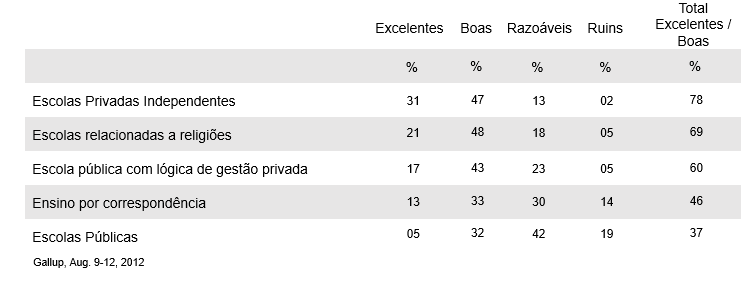
\includegraphics[width=0.8\textwidth]{3-4_binomial_distribution/homeschool.png}
\end{center}
}

\vspace{-30pt}
\soln{
{\footnotesize
\only<2->{
\begin{align*}
\mu &= np = 1,000 \times 0.13 = 130 \\
\sigma &= \sqrt{np(1-p)} = \sqrt{1,000 \times 0.13 \times 0.87} \approx 10.6
\end{align*}
}}}
\vspace{-10pt}
\begin{changemargin}{+1cm}{+0cm}
\pause
\begin{enumerate}
\justifying
\only<3->{\item[Método 1:] Intervalo de observações usuais:\\ $130 \pm 2 \times 10.6 = (108.8, 151.2)$ \\
\justifying
100 está fora desse intervalo, portanto, seria considerado incomum.}
\justifying
\only<4->{\item[Método 2:] Z-score de observação:\\ $Z = \frac{x - mean}{SD} = \frac{100 - 130}{10.6} = -2.83$ \\
100 é mais do que 2 SD abaixo da média, portanto, seria considerado incomum.}
\end{enumerate}
\end{changemargin}

\vfill
\justifying
\ct{\webURL{http://www.gallup.com/poll/156974/private-schools-top-marks-educating-children.aspx}}

\end{frame}
%%%%%%%%%%%%%%%%%%%%%%%%%%%%%%%%%%%

\subsection{Aproximação normal ao binômio}

%%%%%%%%%%%%%%%%%%%%%%%%%%%%%%%%%%%%

\begin{frame}
\frametitle{Formatos de distribuições binomiais}
\justifying
\app{Formatos de distribuições binomiais}
{
\justifying
Para esta atividade, você usará um applet da web. Vá para \webURL{https://gallery.shinyapps.io/dist_calc/} e escolha \textit{Binomial coin experiment} no menu suspenso à esquerda.
\begin{itemize}
\justifying
\item Defina o número de tentativas para 20 e a probabilidade de sucesso para 0,15. Descreva a forma da distribuição do número de sucessos.
\justifying
\item Mantendo $ p $ constante em 0,15, determine o tamanho mínimo de amostra necessário para obter uma distribuição unimodal e simétrica do número de sucessos.
\end{itemize}
}

\end{frame}
%%%%%%%%%%%%%%%%%%%%%%%%%%%%%%%%%%%%

\begin{frame}
\frametitle{Formatos de distribuições binomiais}
\begin{itemize}
\justifying
\item Outras considerações:
\begin{itemize}
\justifying
\item O que acontece com o formato da distribuição quando $ n $ permanece constante e $ p $ muda?
\justifying
\item O que acontece com o formato da distribuição quando $ p $ permanece constante e $ n $ muda?
\end{itemize}
\end{itemize}


\end{frame}

%%%%%%%%%%%%%%%%%%%%%%%%%%%%%%%%%%%%

\begin{frame}
\frametitle{Distribuições do número de sucessos}
\justifying
\dq{Histogramas de amostras do modelo binomial em que $ p = 0,10 $ e $ n = 10 $, $ 30 $, $ 100 $ e $ 300 $. O que acontece quando $ n $ aumenta?}

\begin{center}
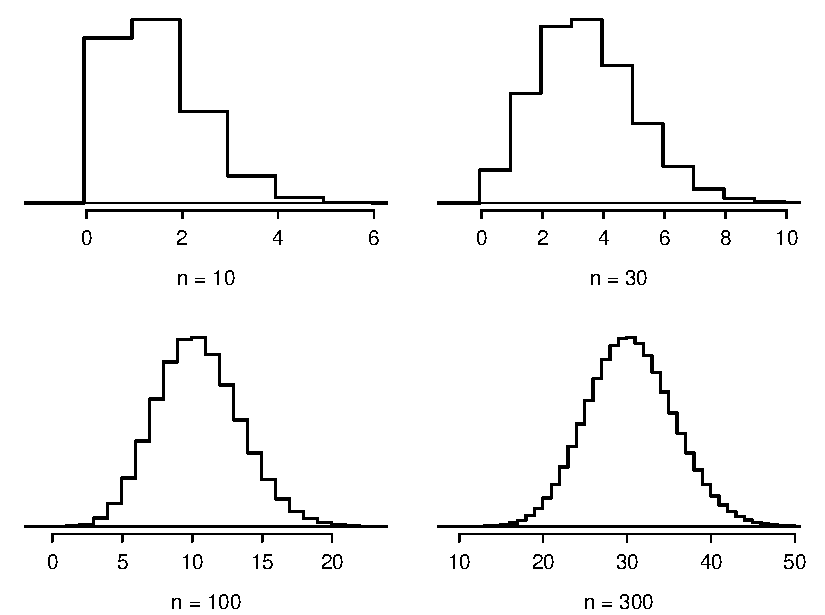
\includegraphics[width=0.60\textwidth]{3-4_binomial_distribution/fourBinomialModelsShowingApproxToNormal.pdf}
\end{center}

\end{frame}

%%%%%%%%%%%%%%%%%%%%%%%%%%%%%%%%%%%

\begin{frame}
\frametitle{Baixo grande é grande o suficiente?}
\justifying
O tamanho da amostra é considerado grande o suficiente se o número esperado de sucessos e fracassos forem pelo menos 10.
\[ np \ge 10 \qquad \text{ e } \qquad n(1-p) \ge 10 \]

\soln{\only<2->{$10 \times 0.13 = 1.3; 10 \times (1 - 0.13) = 8.7$}}

\end{frame}

%%%%%%%%%%%%%%%%%%%%%%%%%%%%%%%%%%

\begin{frame}
\frametitle{Prática}
\justifying
\pq{Abaixo estão quatro pares de parâmetros de distribuição binomial. Qual distribuição pode ser aproximada pela distribuição normal?}

\begin{enumerate}[(a)]
\item $n = 100, p = 0.95$
\solnMult{$n = 25, p = 0.45$} \soln{\only<2>{\orange{$\rightarrow 25 \times 0.45 = 11.25; 25 \times 0.55 = 13.75$}}}
\item $n = 150, p = 0.05$
\item $n = 500, p = 0.015$
\end{enumerate}

\end{frame}


%%%%%%%%%%%%%%%%%%%%%%%%%%%%%%%%%%%%

\begin{frame}
\frametitle{Uma análise dos usuários do Facebook}
\justifying
\dq{Um estudo recente descobriu que "os usuários do Facebook recebem mais do que dão". Por exemplo:
\begin{itemize}
\justifying
\item 40\% dos usuários do Facebook em nossa amostra fizeram uma solicitação de amizade, mas 63\% receberam pelo menos uma solicitação de amizade.
\justifying
\item Os usuários em nossa amostra deram like para o conteúdo dos seus amigos em média 14 vezes, mas tiveram seu conteúdo "curtido" em média 20 vezes.
\justifying
\item Os usuários enviaram 9 mensagens pessoais, mas receberam 12.

\end{itemize}
}
\end{frame}
%%%%%%%%%%%%%%%%%%%%%%%%%%%%%%%%%%%%

\begin{frame}
\frametitle{Uma análise dos usuários do Facebook}
\begin{itemize}
\justifying
\item 12\% dos usuários marcaram um amigo em uma foto, mas 35\% foram marcados em uma foto.
\end{itemize}
\justifying
\hl{Algum palpite de como esse padrão pode ser explicado?}

\justifying
\soln{\only<2>{Usuários ativos contribuem com muito mais conteúdo do que o usuário padrão.}}
\justifying
\ct{\webURL{http://www.pewinternet.org/Reports/2012/Facebook-users/Summary.aspx}}

\end{frame}

%%%%%%%%%%%%%%%%%%%%%%%%%%%%%%%%%%%

\begin{frame}
\frametitle{Prática}
\justifying
\dq{Este estudo também descobriu que aproximadamente 25\% dos usuários do Facebook são considerados usuários ativos. O mesmo estudo descobriu que o usuário médio do Facebook tem 245 amigos. Qual é a probabilidade de que o usuário médio do Facebook com 245 amigos tenha 70 ou mais amigos que seriam considerados usuários ativos? Anote todas as suposições que você fizer.}
\justifying
Temos que $ n = 245, p = 0.25 $ e queremos saber a probabilidade $ P (K \ge 70) $. Para prosseguir, precisamos de independência, o que vamos assumir, mas podemos tentar obter mais dados do Facebook.

\pause
\end{frame}
%%%%%%%%%%%%%%%%%%%%%%%%%%%%%%%%%%%

\begin{frame}
\frametitle{Prática}
\begin{align*}
P(X \ge 70) &= P(K = 70\text{ ou }K = 71\text{ ou }K = 72\text{ ou }\cdots\text{ ou } K = 245) \\
&= P(K = 70) + P(K = 71) + P(K = 72) + \cdots + P(K = 245)
\end{align*}

\pause
\justifying
Isso parece um monte de trabalho ...

\end{frame}

%%%%%%%%%%%%%%%%%%%%%%%%%%%%%%%%%%%%

\begin{frame}
\frametitle{Aproximação normal ao binômio}
\justifying
Quando o tamanho da amostra é grande o suficiente, a distribuição binomial de parâmetros $ n $ e $ p $ pode ser aproximada pelo modelo normal com os parâmetros $ \mu = np $ e $ \sigma = \sqrt {np (1-p)} $.

\begin{itemize}
\justifying
\item No caso dos usuários avançados do Facebook, $n = 245$ e $p = 0.25$.
\[ \mu = 245 \times 0.25 = 61.25 \qquad \sigma = \sqrt{245 \times 0.25 \times 0.75} = 6.78 \]
\justifying
\item $Bin(n = 245, p = 0.25) \approx N(\mu = 61.25, \sigma = 6.78)$.

\begin{center}
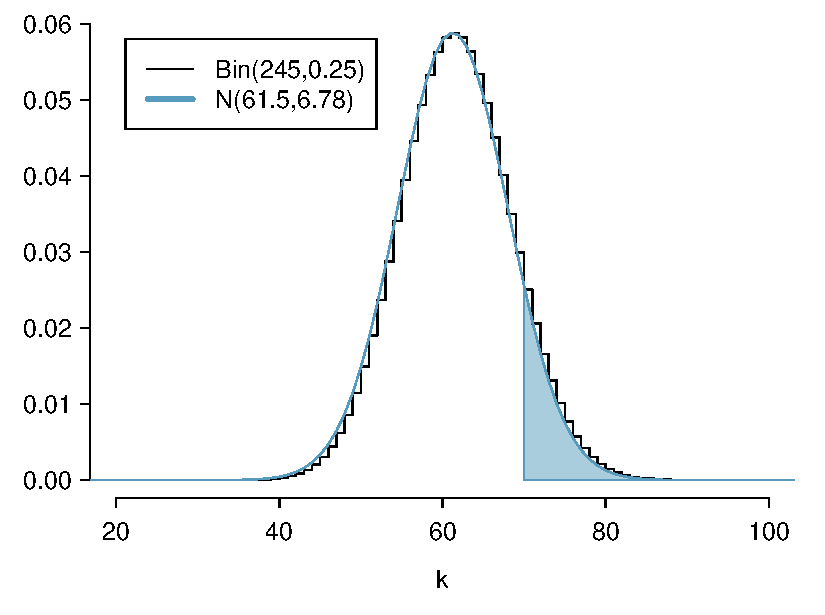
\includegraphics[width=0.4\textwidth]{3-4_binomial_distribution/fb_power_user.pdf}
\end{center}

\end{itemize}

\end{frame}

%%%%%%%%%%%%%%%%%%%%%%%%%%%%%%%%%%%

\begin{frame}
\frametitle{Prática}
\justifying
\dq{Qual é a probabilidade de o usuário médio do Facebook com 245 amigos ter 70 ou mais amigos que seriam considerados usuários avançados?}

\pause

\twocol{0.4}{0.6}{
\begin{center}
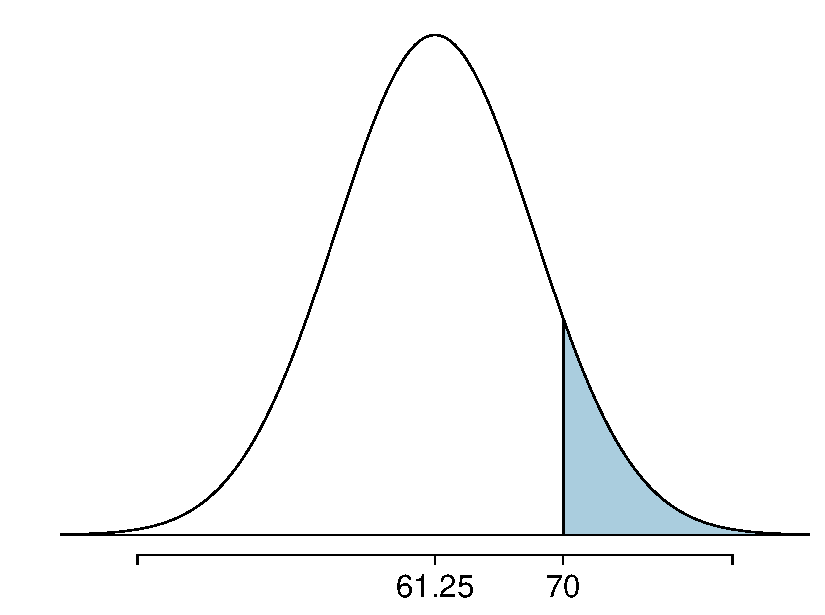
\includegraphics[width=\textwidth]{3-4_binomial_distribution/fb_power_user_norm.pdf}
\end{center}
}
{
\pause
\[ Z = \frac{obs - \textit{média}}{SD} = \frac{70 - 61.25}{6.78} = 1.29 \]

\pause
{\footnotesize
\begin{tabular}{c | rrrr>{\columncolor[gray]{0.6}[0pt]}r |}
  \cline{2-6}
& \multicolumn{5}{c}{Segunda casa decimal de $Z$}  \\
  \cline{2-6}
$Z$ & 0.05 & 0.06 & 0.07 & 0.08 & 0.09   \\
  \hline
  \hline
  1.0 & \tiny{0.8531} & \tiny{0.8554} & \tiny{0.8577} & \tiny{0.8599} & \tiny{0.8621} \\
  1.1 & \tiny{0.8749} & \tiny{0.8770} & \tiny{0.8790} & \tiny{0.8810} & \tiny{0.8830} \\
\rowcolor[gray]{.6}
  1.2 & \tiny{0.8944} & \tiny{0.8962} & \tiny{0.8980} & \tiny{0.8997} & \orange{\tiny{0.9015}} \\  
\end{tabular}
}

\pause
\[ P(Z > 1.29) = 1 - 0.9015 = 0.0985 \]
}

\end{frame}

%%%%%%%%%%%%%%%%%%%%%%%%%%%%%%%%%%


%%%%%%%%%%%%%%%%%%%%%%%%%%%%%%%%%%%%

\section{3.5. Outras distribuições discretas}

%%%%%%%%%%%%%%%%%%%%%%%%%%%%%%%%%%%%

\subsection{Distribuição binomial negativa}

%%%%%%%%%%%%%%%%%%%%%%%%%%%%%%%%%%%%

\begin{frame}
\frametitle{Distribuição binomial negativa}

\begin{itemize}
\justifying
\item O \hl{distribuição binomial negativa} descreve a probabilidade de observar o $ k ^ {esimo} $ sucesso na $ n ^ {esimo} $ tentativa.
\justifying
\item As quatro condições a seguir são úteis para identificar um caso binomial negativo:
\begin{enumerate}
\justifying
\item As tentativas são independentes.
\justifying
\item Cada resultado do estudo pode ser classificado como um sucesso ou fracasso.
\justifying
\item A probabilidade de sucesso ($ p $) é a mesma para cada tentativa.
\justifying
\item A última tentativa deve ser um sucesso.
\end{enumerate}
\justifying
Observe que as três primeiras condições são comuns à distribuição binomial.

\end{itemize}
\end{frame}

%%%%%%%%%%%%%%%%%%%%%%%%%%%%%%%%%%%%

\begin{frame}
\frametitle{Distribuição binomial negativa}

\vfill

\justifying
\formula{Distribuição binomial negativa}
{
P($k^{esimo}$ sucesso na $n^{esimo}$ tentativa) = ${n-1 \choose k-1}~p^k~(1-p)^{n-k}$, \\
\justifying
onde $ p $ é a probabilidade de que uma tentativa individual seja um sucesso. Todas as tentativas são consideradas independentes.
}

\end{frame}

%%%%%%%%%%%%%%%%%%%%%%%%%%%%%%%%%%%%

\begin{frame}
\frametitle{Prática}
\justifying
\dq{Uma estudante universitária que trabalha em um laboratório de psicologia é solicitada a recrutar 10 casais para participar de um estudo. Ela decide ficar do lado de fora do centro estudantil e perguntar a cada 5 pessoas que saem do prédio se eles estão em um relacionamento e, em caso afirmativo, se eles gostariam de participar do estudo com o seu parceiro. Suponha que a probabilidade de encontrar tal pessoa seja 10\%. Qual é a probabilidade da estudante precisar perguntar a 30 pessoas antes de atingir seu objetivo?}

\pause
\justifying
Dado: $ p = 0,10 $, $ k = 10 $, $ n = 30 $. Queremos encontrar a probabilidade do $ 10 ^ {o} $ sucesso na $ 30 ^ {a} $ tentativa, portanto usamos a distribuição binomial negativa.

\pause
\end{frame}
%%%%%%%%%%%%%%%%%%%%%%%%%%%%%%%%%%%%

\begin{frame}
\frametitle{Prática}

\begin{eqnarray*}
P(\text{$10^{o}$ sucesso na $30^{a}$ tentativa}) &=& {29 \choose 9} \times 0.10^{10} \times 0.90^{20} \\
\pause
&=& 10,015,005 \times 0.10^{10} \times 0.90^{20} \\
\pause
&=& 0.00012
\end{eqnarray*}

\end{frame}

%%%%%%%%%%%%%%%%%%%%%%%%%%%%%%%%%%%%

\begin{frame}
\frametitle{Binomial vs. binomial negativo}
\justifying
\dq{Como a distribuição binomial negativa é diferente da distribuição binomial?}

\pause

\begin{itemize}
\justifying
\item No caso binomial, normalmente temos um número fixo de tentativas ao invés de considerar o número de sucessos.
\justifying
\item No caso da binomial negativa, examinamos quantas tentativas são necessárias para observar um número fixo de sucessos, exigindo que a última observação seja um sucesso.

\end{itemize}

\end{frame}

%%%%%%%%%%%%%%%%%%%%%%%%%%%%%%%%%%%%

\begin{frame}
\frametitle{Prática}
\justifying
\pq{Qual das seguintes opções descreve um caso em que usaríamos a distribuição binomial negativa para calcular a probabilidade desejada?}

\begin{enumerate}[(a)]
\justifying
\item Probabilidade de que um menino de 5 anos seja mais alto que 106 centímetros.
\justifying
\item Probabilidade de que 3 de 10 arremessos de softbol sejam bem sucedidos.
\justifying
\item Probabilidade de receber uma sequência de mesmo naipe no poker.
\justifying
\item Probabilidade de perder 8 tiros antes do primeiro acerto.
\justifying
\solnMult{Probabilidade de acertar a bola pela 3 $ ^ {a} $ vez na 8 $ ^ {a} $ tentativa .}

\end{enumerate}

\end{frame}

%%%%%%%%%%%%%%%%%%%%%%%%%%%%%%%%%%%%

\subsection{Distribuição de Poisson}

%%%%%%%%%%%%%%%%%%%%%%%%%%%%%%%%%%%%

\begin{frame}
\frametitle{Distribuição de Poisson}

\begin{itemize}
\justifying
\item A \hl {distribuição de Poisson} é útil para estimar o número de eventos raros por unidade de tempo para uma população grande e fixa, dado que os indivíduos dentro dessa população são independentes.
\justifying
\item A \hl{taxa} para uma distribuição de Poisson é o número médio de ocorrências em uma população fixa por unidade de tempo, e é denotada por \mathhl{\lambda}.
\justifying
\item Usando a taxa, podemos descrever a probabilidade de observar exatamente $ k $ eventos por unidade de tempo.

\end{itemize}

\end{frame}
%%%%%%%%%%%%%%%%%%%%%%%%%%%%%%%%%%%%

\begin{frame}
\frametitle{Distribuição de Poisson}

\vfill
\justifying
\formula{Distribuição de Poisson}
{
P(observar $ k $ eventos) = $\frac{\lambda^k e^{-\lambda}}{k!}$, \\
\vspace{0.5 cm}
\justifying
onde $k$ pode ser 0, 1, 2, e assim por diante, e $k!$ representa $ k $-fatorial. A letra $e \approx 2.718$ é a base do logaritmo natural. \\
\vspace{0.5 cm}
\justifying
A média e o desvio-padrão dessa distribuição são $ \lambda $ e $ \sqrt{\lambda} $, respectivamente.
}

\end{frame}

%%%%%%%%%%%%%%%%%%%%%%%%%%%%%%%%%%%%

\begin{frame}
\frametitle{Prática}
\justifying
\dq{Suponha que falhas de energia elétrica ocorram em uma região rural de um país em desenvolvimento, seguindo uma distribuição de Poisson com média de 2 falhas a cada semana. \\
Calcule a probabilidade de que, em uma determinada semana, a eletricidade falhe apenas uma vez.}

\pause
\justifying
Dado $\lambda = 2$.

\pause

\begin{eqnarray*}
P(\text{apenas 1 falha em uma semana}) &=& \frac{2^1 \times e^{-2}}{1!} \\
\pause
&=& \frac{2 \times e^{-2}}{1} \\
\pause
&=& 0.27
\end{eqnarray*}

\end{frame}

%%%%%%%%%%%%%%%%%%%%%%%%%%%%%%%%%%%%

\begin{frame}
\frametitle{Prática}
\justifying
\dq{Suponha que falhas de energia elétrica ocorram em uma região rural de um país em desenvolvimento, seguindo uma distribuição de Poisson com média de 2 falhas a cada semana. \\
Calcule a probabilidade de que em um determinado \underline{dia} a eletricidade falhe três vezes.}

\pause
\justifying
Temos a taxa de falha semanal, mas para responder a essa pergunta precisamos primeiro calcular a taxa média de falha em um determinado dia: $\lambda_{dia} = \frac{2}{7} = 0.2857$. Note que estamos assumindo que a probabilidade de falha de energia é a mesma em qualquer dia da semana, ou seja, assumimos independência.


\end{frame}
%%%%%%%%%%%%%%%%%%%%%%%%%%%%%%%%%%%%

\begin{frame}
\frametitle{Prática}

\begin{eqnarray*}
P(\text{3 falhas em um determinado dia}) &=& \frac{0.2857^1 \times e^{-0.2857}}{3!} \\
\pause
&=& \frac{0.2857 \times e^{-0.2857}}{6} \\
\pause
&=& 0.0358
\end{eqnarray*}

\end{frame}

%%%%%%%%%%%%%%%%%%%%%%%%%%%%%%%%%%%%

\begin{frame}
\frametitle{É Poisson?}

\begin{itemize}
\justifying
\item Uma variável aleatória pode seguir uma distribuição de Poisson se o evento que está sendo considerado for raro, a população for grande e os eventos ocorrerem independentemente um do outro.
\justifying
\item No entanto, podemos pensar em situações em que os eventos não são realmente independentes. Por exemplo, se estivermos interessados na probabilidade de um certo número de casamentos durante um verão, devemos levar em consideração que fins de semana são mais populares para casamentos.
\justifying
\item Nesse caso, um modelo de Poisson pode às vezes ainda ser razoável se permitirmos que ele tenha uma taxa diferente para tempos diferentes; poderíamos modelar a taxa como maior nos finais de semana do que nos dias da semana.
\end{itemize}

\end{frame}
%%%%%%%%%%%%%%%%%%%%%%%%%%%%%%%%%%%%

\begin{frame}
\frametitle{É Poisson?}

\begin{itemize}
\justifying
\item A ideia de modelar taxas para uma distribuição de Poisson em relação a uma segunda variável (dia da semana) forma a base de alguns métodos mais avançados chamados \hl{modelos lineares generalizados}. Isso vai além do escopo deste curso, mas discutiremos uma base de modelos lineares nos Capítulos 7 e 8.

\end{itemize}

\end{frame}

%%%%%%%%%%%%%%%%%%%%%%%%%%%%%%%%%%%%

\begin{frame}
\frametitle{Prática}
\justifying
\pq{Qual variável aleatória que segue as seguintes distribuições pode assumir valores diferentes de inteiros positivos?}

\begin{enumerate}[(a)]
\item Poisson
\item Binomial negativo
\item Binomial
\solnMult{Normal}
\item Geométrico
\end{enumerate}

\end{frame}
%%%%%%%%%%%%%%%%%%%%



%%%%%%%%%%%%%%%%%%%%%%%%%%%%%%%%%%%%
% End document
%%%%%%%%%%%%%%%%%%%%%%%%%%%%%%%%%%%%

\end{document}